\documentclass[11pt]{article}
\usepackage{amsmath,amssymb,amsthm,mathtools,bm}
\usepackage[margin=1in]{geometry}
\usepackage{booktabs,tabularx,array}
\usepackage{algorithm}
\usepackage{algorithmic}
\usepackage[hidelinks]{hyperref}
\usepackage{enumitem}
\usepackage{xcolor}
\usepackage{microtype}
\usepackage{graphicx}
\usepackage{tikz}
\usetikzlibrary{positioning,arrows.meta,calc,fit,backgrounds}


\newtheorem{theorem}{Theorem}
\newtheorem{proposition}{Proposition}
\newtheorem{corollary}{Corollary}
\newtheorem{lemma}{Lemma}
\newtheorem{assumption}{Assumption}
\newtheorem{remark}{Remark}
\newcommand{\PP}{\mathbb{P}}
\newcommand{\EE}{\mathbb{E}}
\newcommand{\RR}{\mathbb{R}}
\newcommand{\ind}{\mathbf{1}}
\newcommand{\calA}{\mathcal{A}}
\newcommand{\calC}{\mathcal{C}}
\newcommand{\calF}{\mathcal{F}}
\newcommand{\riskhat}{\widehat R}
\newcommand{\R}{\mathbb{R}}
\newcommand{\Reg}{\operatorname{Reg}}
\DeclareMathOperator*{\argmax}{arg\,max}
\DeclareMathOperator*{\argmin}{arg\,min}
\newtheorem{definition}{Definition}

\title{Trajectory-Level Risk Allocation for Multi-Horizon Online Conformal Prediction\\\large Dependence Learning, Right-Censored Feedback, and Online Guarantees}
\author{}
\date{}

\begin{document}
\begin{center}
{\Large\bfseries Trajectory-Level Risk Allocation for Multi-Horizon Online Conformal Prediction}\par
\vspace{2pt}
{\normalsize Dependence Learning, Right-Censored Feedback, and Online Guarantees}
\end{center}
\vspace{-0.5em}

\section*{One-page problem summary}
\footnotesize
\noindent
\textbf{Objective.}
At forecast origin $k$, issue $H$ nested prediction sets
$\{\mathcal C_{k,h}(\alpha_{k,h})\}_{h=1}^H$.  Let
\[
    V_{k,h}
    :=
    \mathbf 1\{Y_{k+h}\notin\mathcal C_{k,h}(\alpha_{k,h})\},
    \qquad
    Z_k:=\max_{1\le h\le H}V_{k,h}.
\]
The primary validity objective is whole-trajectory calibration,
\[
    \frac1K\sum_{k=1}^K Z_k\longrightarrow\beta,
\]
while the primary efficiency objective is low regret relative to an
oracle trajectory-risk allocator.

\smallskip
\noindent
\textbf{Outer calibration state and common risk resource.}
Each trajectory contributes exactly one binary outcome $Z_k$.  Its label is
processed when it becomes known: at the first violation if the trajectory
fails, or at horizon $H$ if it succeeds.  A scalar state $q_t$ carries the
exact resolved-label accounting,
\[
    q_t
    =
    q_{t-1}
    +
    \eta\sum_{k\in\mathcal R_t}(\beta-Z_k).
\]
On ordinary rounds, a predictable outer controller proposes a scalar
trajectory-risk budget $\widetilde b_t\in[0,1]$ from the available feedback
signal.  The exact state $q_t$ acts as a safety wrapper: outside fixed state
thresholds the algorithm uses formal conservative/aggressive extreme actions,
while inside the safe region it exposes $b_t=\widetilde b_t$ to the inner
allocator.  The clipped affine map $\widetilde b_t=\phi(q_t)$ is the simplest
baseline.  Thus $\beta$ remains fixed, $q_t$ carries validity accounting, and
$b_t$ is the resource seen by the optimizer.

\smallskip
\noindent
\textbf{Dependence-aware allocation.}
Given $b_t$, horizon-specific marginal miscoverage levels are selected by
\[
\boxed{
\bm\alpha_t\in\argmax_{\bm\alpha\in\mathcal A}
\sum_{h=1}^H U_{t,h}(\alpha_h)
\quad\text{s.t.}\quad
\widehat R_t(\bm\alpha)\le b_t .}
\]
For a predictable fixed forest $F_t$,
\[
    \widehat R_t(\bm\alpha)
    =
    \sum_{h=1}^H\alpha_h
    -
    \sum_{e=(s,r)\in F_t}
    \widetilde p_{t,e}(\alpha_s,\alpha_r),
\]
where $\widetilde p_{t,e}$ is a conservative lower certificate for simultaneous
failure probability.  The dependence term is therefore an
allocation-dependent risk rebate, not an additional scalar budget.

\smallskip
\noindent
\textbf{Why right-censoring matters.}
A failed trajectory is known at its first violation, while a successful
trajectory is known only after all $H$ horizons survive.  Nevertheless at most
$H$ issued trajectories are unresolved at any physical time.  This yields the
pathwise accounting bound
\[
    \left|
        \frac1T\sum_{k=1}^T(Z_k-\beta)
    \right|
    \le
    \frac{|q_T-q_0|}{\eta T}
    +
    \frac HT.
\]
With extreme prediction-set safeguards, the latent state is uniformly bounded,
so for fixed $H$ the trajectory-calibration error is $\mathcal O(T^{-1})$.

\smallskip
\noindent
\textbf{Two performance criteria.}
All statistical, numerical, delay, forest-selection, and shape-approximation
errors are treated as contributors to one of two headline quantities:
\[
    \boxed{
    \operatorname{Reg}^{\mathrm{opt}}_T
    }
    \qquad\text{and}\qquad
    \boxed{
    \operatorname{Cal}_T
    :=
    \frac1T\sum_{k=1}^T(Z_k-\beta).
    }
\]
The first measures efficiency relative to an oracle allocator under the same
outer budget sequence; the second measures realized trajectory-level coverage.
On the simultaneous dependence-certification event, stable dependence,
bounded risk prices, and vanishing cumulative approximation error imply
sublinear optimization regret.  Shape loss is not a
third metric: it is one possible contribution to
$\operatorname{Reg}^{\mathrm{opt}}_T$.
\normalsize

\clearpage
\section*{Information flow}
\begin{figure}[h!]
\centering
\resizebox{0.98\textwidth}{!}{%
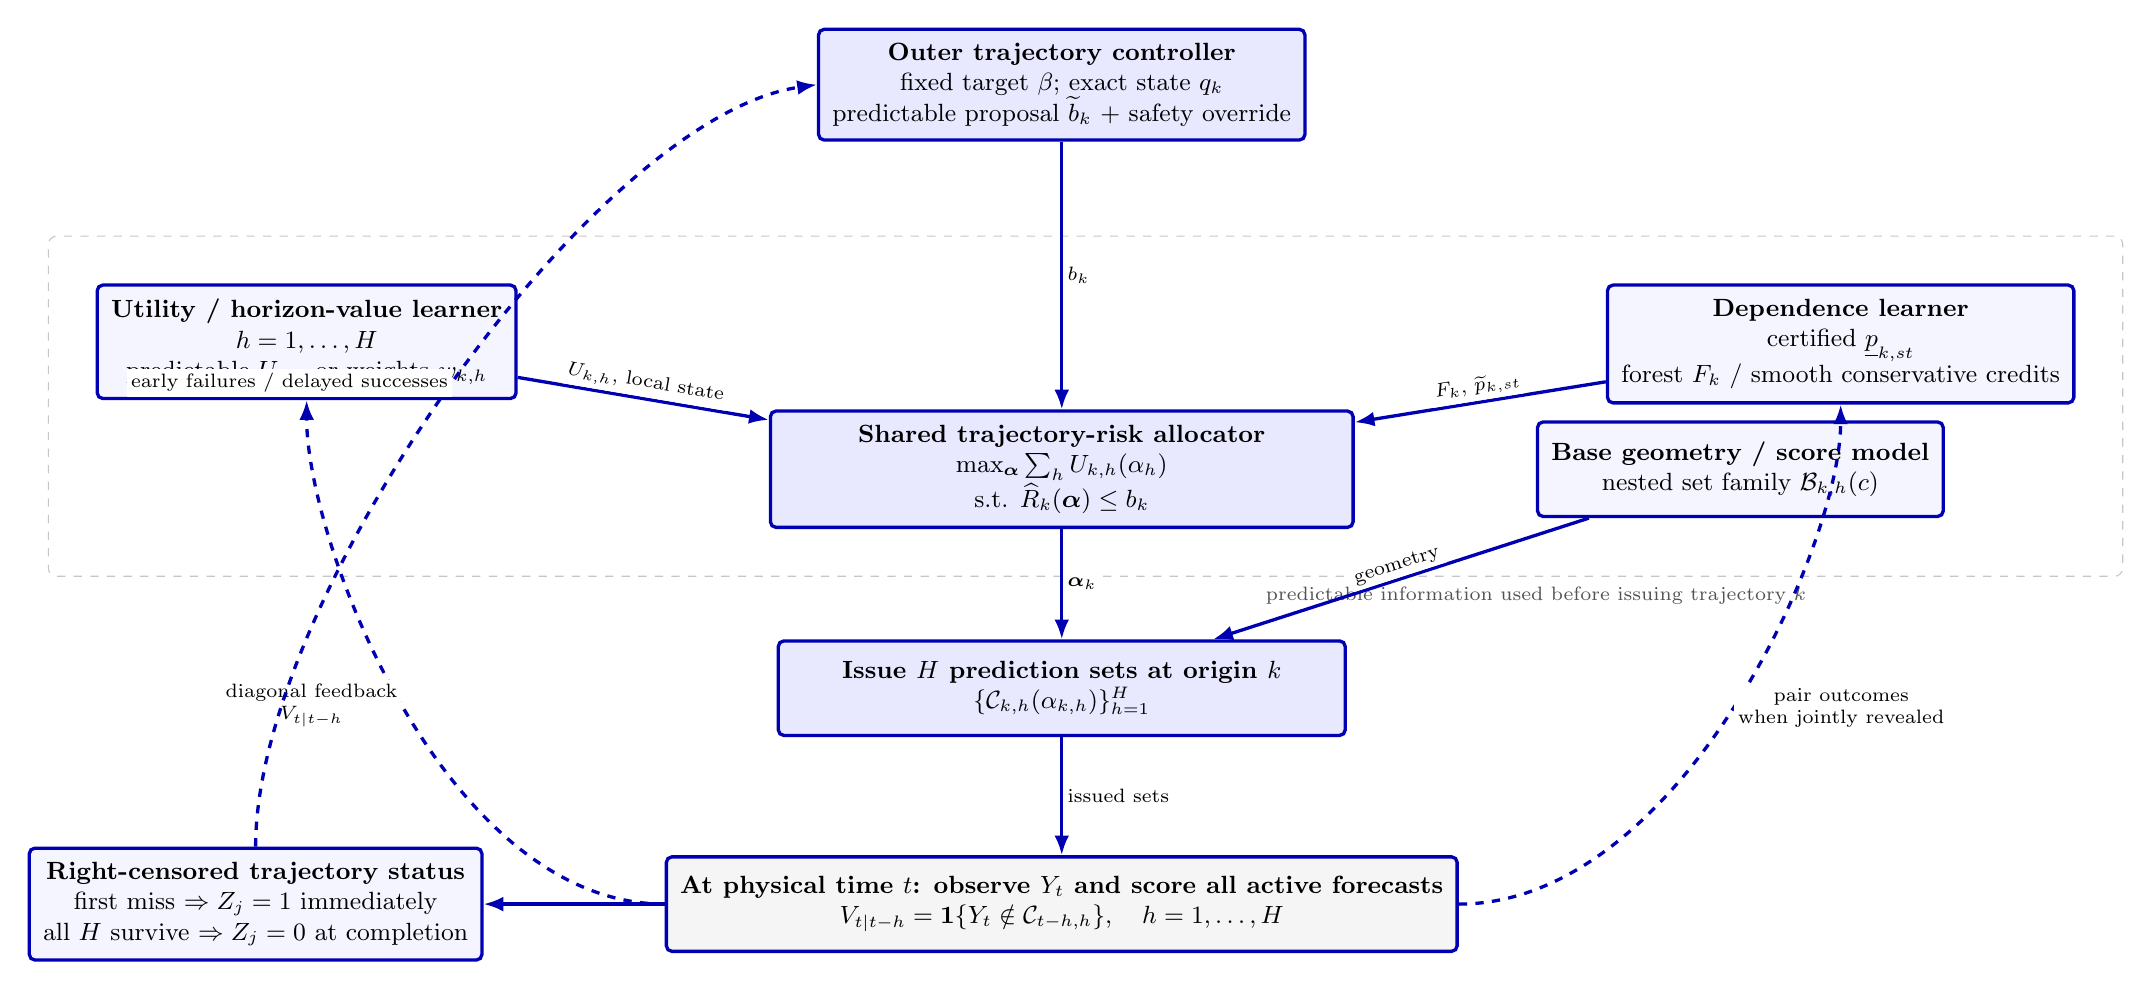
\begin{tikzpicture}[
    font=\small,
    node distance=10mm and 13mm,
    box/.style={draw=blue!70!black, rounded corners=2pt, very thick, align=center, fill=blue!4, minimum height=12mm, inner sep=5pt},
    main/.style={box, fill=blue!9, minimum width=50mm},
    side/.style={box, minimum width=45mm},
    obs/.style={box, fill=gray!8, minimum width=63mm},
    arr/.style={-{Latex[length=2.5mm]}, very thick, draw=blue!70!black},
    darr/.style={-{Latex[length=2.5mm]}, very thick, dashed, draw=blue!70!black},
    lab/.style={font=\scriptsize, align=center, fill=white, inner sep=1.5pt}
]

\node[main] (outer) {\textbf{Outer trajectory controller}\\fixed target $\beta$; exact state $q_k$\\predictable proposal $\widetilde b_k$ + safety override};
\node[side, below left=18mm and 38mm of outer] (horizon) {\textbf{Utility / horizon-value learner}\\$h=1,\ldots,H$\\predictable $U_{k,h}$ or weights $w_{k,h}$};
\node[side, below right=18mm and 38mm of outer] (dep) {\textbf{Dependence learner}\\certified $\underline p_{k,st}$\\forest $F_k$ / smooth conservative credits};
\node[main, below=34mm of outer, minimum width=74mm] (alloc) {\textbf{Shared trajectory-risk allocator}\\$\max_{\bm\alpha}\sum_h U_{k,h}(\alpha_h)$\\s.t. $\widehat R_k(\bm\alpha)\le b_k$};
\node[side, right=23mm of alloc] (geom) {\textbf{Base geometry / score model}\\nested set family $\mathcal B_{k,h}(c)$};
\node[main, below=14mm of alloc, minimum width=72mm] (sets) {\textbf{Issue $H$ prediction sets at origin $k$}\\$\{\mathcal C_{k,h}(\alpha_{k,h})\}_{h=1}^H$};
\node[obs, below=15mm of sets] (check) {\textbf{At physical time $t$: observe $Y_t$ and score all active forecasts}\\$V_{t\mid t-h}=\mathbf 1\{Y_t\notin\mathcal C_{t-h,h}\},\quad h=1,\ldots,H$};
\node[side, left=23mm of check] (censor) {\textbf{Right-censored trajectory status}\\first miss $\Rightarrow Z_j=1$ immediately\\all $H$ survive $\Rightarrow Z_j=0$ at completion};

\draw[arr] (outer) -- node[lab, right] {$b_k$} (alloc);
\draw[arr] (horizon) -- node[lab, above, sloped] {$U_{k,h}$, local state} (alloc);
\draw[arr] (dep) -- node[lab, above, sloped] {$F_k$, $\widetilde p_{k,st}$} (alloc);
\draw[arr] (alloc) -- node[lab, right] {$\bm\alpha_k$} (sets);
\draw[arr] (geom) -- node[lab, above, sloped] {geometry} (sets);
\draw[arr] (sets) -- node[lab, right] {issued sets} (check);
\draw[arr] (check) -- (censor);

\draw[darr] (check.west) .. controls +(-28mm,0mm) and +(0,-18mm) ..
    node[lab, left] {diagonal feedback\\$V_{t\mid t-h}$} (horizon.south);
\draw[darr] (check.east) .. controls +(28mm,0mm) and +(0,-18mm) ..
    node[lab, right] {pair outcomes\\when jointly revealed} (dep.south);
\draw[darr] (censor.north) .. controls +(0,32mm) and +(-28mm,-4mm) ..
    node[lab, left] {early failures / delayed successes} (outer.west);

\begin{scope}[on background layer]
\node[draw=gray!45, rounded corners=3pt, dashed, fit=(horizon)(dep)(alloc), inner sep=6mm,
      label={[font=\scriptsize, text=gray!65!black]below right:predictable information used before issuing trajectory $k$}] {};
\end{scope}
\end{tikzpicture}%
}
\caption{Information flow for the proposed multi-horizon online conformal architecture. A single physical observation resolves one horizon-specific error for each active forecast origin. These shared observations update horizon learners and dependence estimates, while trajectory-level failures are revealed early and successes only after the full horizon. The common risk allocator combines the safeguarded scalar budget, horizon utilities, and certified dependence credit before a warm-started SQP/RTI step issues the next trajectory.}
\label{fig:information-flow}
\end{figure}

\clearpage
\section{Motivation}

Consider a forecaster that, at physical time $k$, issues prediction sets for the next $H$ outcomes. The $h$th set predicts $Y_{k+h}$ and is denoted
\[
    \calC_{k,h}(\alpha_{k,h}),\qquad h=1,\ldots,H,
\]
where $\alpha_{k,h}$ is a horizon-specific marginal miscoverage allocation. Larger $\alpha_{k,h}$ typically permits a smaller prediction set, so marginal risk is a scarce resource that can be exchanged for efficiency.

The desired trajectory event is not an average of marginal errors. It is whole-trajectory containment. Define
\begin{equation}
    V_{k,h}
    :=
    \ind\{Y_{k+h}\notin \calC_{k,h}(\alpha_{k,h})\},
    \qquad
    Z_k
    :=
    \max_{1\le h\le H}V_{k,h}.
    \label{eq:trajectory-failure}
\end{equation}
Thus $Z_k=1$ if at least one member of the $H$-step trajectory falls outside its issued prediction set. The long-run target is
\begin{equation}
    \frac{1}{K}\sum_{k=1}^K Z_k \approx \beta,
    \label{eq:trajectory-target}
\end{equation}
where $\beta$ is the desired trajectory-level miscoverage rate.

A uniform allocation $\alpha_{k,1}=\cdots=\alpha_{k,H}$ is generally wasteful. Different horizons have different predictive difficulty, different delays before their feedback is revealed, and different dependence relationships with the rest of the trajectory. The central design question is therefore:

\begin{quote}
How should a common trajectory-level risk budget be allocated across horizons so that prediction sets are efficient, while the collection of allocations remains jointly compatible with the desired trajectory coverage?
\end{quote}

\section{Architecture and separation of roles}
\label{sec:architecture}

The framework separates four objects that should not be conflated.

\paragraph{Exact trajectory-level accounting.}
The desired trajectory miscoverage $\beta$ is fixed.  A scalar state $q_t$
accumulates only resolved trajectory-level coverage credit/debt.  This state is
model free and is the object used in the pathwise calibration proof.

\paragraph{Ordinary-round actuation.}
A predictable feedback construction produces an ordinary-round control signal.
A controller---for example a fixed-gain ACI update, a DtACI-style adaptive-gain
scheme, or another stable scalar controller---maps that signal to a proposed
budget $\widetilde b_t\in[0,1]$.  The exact state $q_t$ supplies a separate
safety override, producing the budget $b_t$ that is actually exposed to the
inner allocator.  The baseline $\widetilde b_t=\phi(q_t)$ is recovered as a
special case.

\paragraph{Horizon-specific value of risk.}
Each horizon $h$ has a predictable utility function
\[
    U_{t,h}:\calA_h\to\RR,
\]
where $U_{t,h}(\alpha)$ quantifies the benefit of allocating marginal
miscoverage $\alpha$ to that horizon.  The utility may encode prediction-set
width, volume, a downstream control objective, or a learned surrogate.  In the
proportional-fair specialization, its horizon weights may evolve slowly from
set-size and first-failure information.

\paragraph{Trajectory-risk charge.}
The vector $\bm\alpha_t=(\alpha_{t,1},\ldots,\alpha_{t,H})$ incurs a certified
trajectory-risk charge
\[
    \riskhat_t(\bm\alpha_t).
\]
This charge combines marginal risk with dependence information and determines
which allocations are feasible:
\[
    \riskhat_t(\bm\alpha_t)\le b_t.
\]

The separation is deliberate.  The outer controller determines \emph{how much}
trajectory risk may be spent; the utility determines \emph{where that risk is
valuable}; the dependence certificate determines \emph{how expensive} a
candidate allocation is to whole-trajectory containment; and the exact state
$q_t$ remains the validity backbone.

\section{General trajectory-risk allocation problem}
\label{sec:general}

Let
\[
    \calA=\calA_1\times\cdots\times\calA_H
\]
be the feasible set of horizon allocations. The general inner problem is
\begin{equation}
\boxed{
\begin{aligned}
    \max_{\bm\alpha\in\calA}\quad
        & \sum_{h=1}^H U_{k,h}(\alpha_h)\\
    \text{s.t.}\quad
        & \riskhat_k(\bm\alpha)\le b_k.
\end{aligned}}
\label{eq:general-allocation}
\end{equation}

The formulation is intentionally agnostic about how $U_{k,h}$ and $\riskhat_k$ are learned. It only requires that they be determined from information available when the allocation is selected.

\subsection{Dependence-aware trajectory risk}

Suppose the marginal calibration layer supplies the horizon-wise charges $\alpha_h$, and suppose that for selected horizon pairs $(s,t)$ we have certified lower bounds
\begin{equation}
    \underline p_{k,st}(\alpha_s,\alpha_t)
    \le
    \PP(V_{k,s}=1,V_{k,t}=1)
    \label{eq:pair-lower-bound}
\end{equation}
under the conditioning/validity regime used by the calibration theorem. For a forest $F_k$ on the horizon indices, Hunter's second-order union inequality gives the certified risk surrogate
\begin{equation}
    \riskhat_{k,F_k}(\bm\alpha)
    :=
    \sum_{h=1}^H \alpha_h
    -
    \sum_{(s,t)\in F_k}
    \underline p_{k,st}(\alpha_s,\alpha_t).
    \label{eq:forest-risk}
\end{equation}
The first term is the Boole charge. The second term is certified overlap credit. Hence dependence learning does not create additional risk budget; it prevents the allocator from paying twice for failures that are known to occur together.

For the optimization layer, it is useful to treat the forest $F_k$ as fixed while solving \eqref{eq:general-allocation}. It may be selected from predictable, certified information immediately before the allocation problem is solved. Jointly re-selecting the maximum-weight forest as a function of $\bm\alpha$ generally creates additional nonsmooth/nonconvex structure; Section~\ref{sec:convexity} therefore freezes the forest inside each SQP solve.

\subsection{A game-theoretic interpretation}

Associate a nonnegative dual price $\lambda_k$ with the common trajectory budget. The Lagrangian is
\begin{equation}
    \mathcal L_k(\bm\alpha,\lambda)
    =
    -\sum_{h=1}^H U_{k,h}(\alpha_h)
    +
    \lambda\bigl(\riskhat_k(\bm\alpha)-b_k\bigr).
    \label{eq:general-lagrangian}
\end{equation}
Each horizon behaves like an agent requesting risk from a common resource. The utility term rewards receiving additional marginal risk when doing so improves efficiency. The dual variable $\lambda_k$ is the shadow price of trajectory risk. Dependence modifies the effective price paid by each horizon through its marginal contribution to $\riskhat_k$.

At an interior differentiable solution,
\begin{equation}
    U'_{k,h}(\alpha_{k,h})
    =
    \lambda_k
    \frac{\partial \riskhat_k}{\partial\alpha_h}(\bm\alpha_k).
    \label{eq:general-kkt}
\end{equation}
Equation~\eqref{eq:general-kkt} captures the desired allocation principle: a horizon should receive more risk when the marginal utility is high or when an additional unit of its marginal risk contributes relatively little to whole-trajectory failure.

\section{Fixed-forest inner optimization: SQP and an optional convex relaxation}
\label{sec:convexity}

The fixed-forest allocation problem is generally nonconvex.  Coordinatewise
monotonicity of an overlap surface does not imply concavity, so requiring a
global concave minorant solely to obtain convexity can discard substantial
dependence credit.  The primary computational method in this paper is therefore
a smooth conservative nonlinear program solved by warm-started sequential
quadratic programming (SQP), or by one SQP real-time iteration when the sampling
rate requires it.

\begin{assumption}[Smooth certified SQP model]
\label{ass:sqp-model}
For round $k$:
\begin{enumerate}[leftmargin=*]
    \item $\calA$ is a compact box with
    $0<\alpha_{\min}\le\alpha_h\le\alpha_{\max}<1$;
    \item each $U_{k,h}$ is twice continuously differentiable on $\calA_h$;
    \item the forest $F_k$ is selected predictably and held fixed during the
    nonlinear solve;
    \item for every $e\in F_k$, the optimization surface
    $\widetilde p_{k,e}$ is twice continuously differentiable on the region
    queried by the solver and is conservative:
    \[
        \widetilde p_{k,e}(\bm\alpha_e)
        \le
        \underline p_{k,e}(\bm\alpha_e)
        \le
        p_{k,e}(\bm\alpha_e).
    \]
\end{enumerate}
\end{assumption}

Define
\begin{equation}
    \widetilde R_{k,F_k}(\bm\alpha)
    :=
    \sum_{h=1}^H\alpha_h
    -
    \sum_{e\in F_k}\widetilde p_{k,e}(\bm\alpha_e).
    \label{eq:sqp-risk-surface}
\end{equation}
The ordinary inner problem is
\begin{equation}
\boxed{
\begin{aligned}
    \max_{\bm\alpha\in\calA}\quad
        & \sum_{h=1}^H U_{k,h}(\alpha_h)\\
    \text{s.t.}\quad
        & \widetilde R_{k,F_k}(\bm\alpha)\le b_k.
\end{aligned}}
\label{eq:sqp-inner-problem}
\end{equation}
No concavity assumption is imposed on $\widetilde p_{k,e}$ in the primary
method.  A feasible SQP output is sufficient for validity because replacing the
true overlap by a pointwise lower surface only increases the Hunter risk
surrogate.  Global optimality affects efficiency, not coverage.

In implementation, the previous primal-dual solution is used as the warm start,
the forest and learned surfaces are frozen during the solve, and the returned
allocation is checked against
\[
    \widetilde R_{k,F_k}(\bm\alpha_k)\le b_k
\]
before the prediction sets are issued.  If the final iterate violates the
constraint beyond numerical tolerance, the round is repaired or rejected in
favor of a certified feasible allocation.

\paragraph{Why freeze the forest?}
If
\[
    W_k(\bm\alpha)
    =
    \max_{F\in\mathcal F}
    \sum_{e\in F}\widetilde p_{k,e}(\bm\alpha_e),
\]
then changing the maximizing forest as $\bm\alpha$ moves introduces a
piecewise-defined objective/constraint surface and can change the active
combinatorial structure inside the nonlinear solve.  We therefore select
$F_k$ immediately before optimization and hold it fixed for that round.  A
suboptimal certified forest affects efficiency but not validity.

\paragraph{Optional convex relaxation.}
A globally convex inner problem remains available when desired.  Suppose, in
addition to the conditions above, that each $U_{k,h}$ is concave and each
$\widetilde p_{k,e}$ is a concave conservative lower bound.  Then
$-\widetilde p_{k,e}$ is convex and
$\widetilde R_{k,F_k}$ is convex.  Hence
\[
    \{\bm\alpha\in\calA:\widetilde R_{k,F_k}(\bm\alpha)\le b_k\}
\]
is convex and maximizing the concave utility is a convex optimization problem.
This relaxation is useful as a benchmark or fallback, but any additional loss
of overlap credit caused by concavification is treated as approximation error
in the efficiency analysis rather than as a validity requirement.

\section{Specific instantiation: proportional-fair risk allocation}
\label{sec:pf}

A particularly simple utility is weighted proportional fairness:
\begin{equation}
    U_{k,h}(\alpha_h)
    =
    w_{k,h}\log \alpha_h,
    \qquad
    w_{k,h}>0.
    \label{eq:log-utility}
\end{equation}
We restrict
\[
    0<\alpha_{\min}\le\alpha_h\le\alpha_{\max}<1
\]
to avoid degeneracy and to encode any practical marginal-risk limits. The concrete inner problem is
\begin{equation}
\boxed{
\begin{aligned}
    \max_{\bm\alpha}\quad
        & \sum_{h=1}^H w_{k,h}\log\alpha_h\\
    \text{s.t.}\quad
        & \sum_{h=1}^H\alpha_h
        -\sum_{(s,t)\in F_k}
        \widetilde p_{k,st}(\alpha_s,\alpha_t)
        \le b_k,\\
        & \alpha_{\min}\le\alpha_h\le\alpha_{\max},
        \qquad h=1,\ldots,H.
\end{aligned}}
\label{eq:pf-allocation}
\end{equation}
In the primary implementation, \eqref{eq:pf-allocation} is a smooth fixed-forest nonlinear program solved by warm-started SQP.  It becomes convex under the optional concave-overlap relaxation described in Section~\ref{sec:convexity}.

The logarithm provides an anti-starvation mechanism. Sending any horizon toward zero marginal risk incurs an increasingly large utility penalty. The weights $w_{k,h}$ encode the predictable horizon-specific value of additional marginal risk.  They may be fixed exogenously or adapted online from prediction-set efficiency and first-failure information as described in Section~\ref{sec:adaptive-utility-weights}.
\subsection{Marginal risk price}

Ignoring active box constraints, the KKT stationarity condition for \eqref{eq:pf-allocation} is
\begin{equation}
    \frac{w_{k,h}}{\alpha_{k,h}}
    =
    \lambda_k
    \left[
        1-
        \sum_{e\in F_k:e\ni h}
        \frac{\partial\widetilde p_{k,e}}{\partial\alpha_h}
    \right].
    \label{eq:pf-kkt}
\end{equation}
The bracketed term is the marginal certified trajectory-risk charge for horizon $h$. Thus a horizon receives more marginal risk when either its weight $w_{k,h}$ is large or its additional failures overlap strongly with failures already represented by the forest.

Equation~\eqref{eq:pf-kkt} gives a useful economic interpretation. The allocation does not ask whether horizon $h$ is difficult in isolation. It asks how much efficiency is gained per unit of \emph{incremental trajectory risk}. Two horizons can have identical marginal error behavior and nevertheless receive different allocations because their dependence with the rest of the trajectory differs.

\subsection{Relation to direct set-size minimization}

If a differentiable set-size function $S_{k,h}(\alpha)$ is available and is convex and decreasing in $\alpha$, another principled choice is
\[
    U_{k,h}(\alpha)=-\omega_{k,h}S_{k,h}(\alpha).
\]
Then \eqref{eq:general-allocation} directly minimizes weighted total set size. The proportional-fair utility \eqref{eq:log-utility} is useful when a stable convex model of set size is unavailable or when explicit anti-starvation is desirable.

\subsection{Adaptive horizon utility weights}
\label{sec:adaptive-utility-weights}

The outer budget $b_t$ controls how much total trajectory risk is available;
the utility weights $\bm w_t=(w_{t,1},\ldots,w_{t,H})$ control where that risk is
valuable.  The two feedback loops are intentionally separate.  Calibration
errors act on the outer budget, whereas efficiency and horizon fragility may
act on the utility weights.

For proportional-fair utility,
\[
    U_t(\bm\alpha)
    =
    \sum_{h=1}^H w_{t,h}\log\alpha_h,
    \qquad
    \frac{\partial U_t}{\partial\alpha_h}
    =
    \frac{w_{t,h}}{\alpha_h}.
\]
Thus increasing $w_{t,h}$ tends to allocate more marginal risk to horizon $h$.
A horizon that is frequently the first location of trajectory failure should
therefore not automatically receive more weight.

\paragraph{Static weights.}
Let $c_h>0$ denote application-level horizon importance.  The simplest choice is
\begin{equation}
    w_{t,h}
    =
    \frac{c_h}{\sum_{j=1}^H c_j}.
    \label{eq:static-utility-weights}
\end{equation}
This remains the default when no online utility adaptation is desired.

\paragraph{Marginal efficiency.}
Let $S_{t,h}(a)$ denote a predictable set-size or efficiency cost at marginal
miscoverage $a$; examples include interval width, set volume, or an
application-specific burden.  Define
\begin{equation}
    m_{t,h}(a)
    :=
    -\frac{\partial S_{t,h}(a)}{\partial a}\ge0.
    \label{eq:marginal-set-efficiency}
\end{equation}
If an analytic derivative is unavailable, estimate it on the marginal-risk
grid by a centered finite difference or a smooth interpolant.  Matching the
local slope of $-c_hS_{t,h}(\alpha_h)$ to the log-utility slope gives the raw
efficiency target
\begin{equation}
\boxed{
    w_{t,h}^{\mathrm{eff}}
    :=
    c_h\alpha_{t-1,h}\widehat m_{t,h},
    \qquad
    \widehat m_{t,h}:=m_{t,h}(\alpha_{t-1,h}).
}
\label{eq:efficiency-target-weight}
\end{equation}
Thus the numerically convenient log utility can locally track the direct
set-size objective while retaining its anti-starvation behavior.

\paragraph{Optional failure-aware weighting.}
Let $\tau_k$ denote the first-failure horizon, with $\tau_k=\infty$ for a
successful trajectory; Section~\ref{sec:right-censored-feedback} formalizes
this quantity.  A censoring-safe recent estimate of first-failure mass uses
only fully resolved origins:
\begin{equation}
    \widehat f_{t,h}^{(W)}
    :=
    \frac1W
    \sum_{k=t-H-W+1}^{t-H}
    \mathbf 1\{\tau_k=h\}.
    \label{eq:first-failure-mass-estimator}
\end{equation}
Because every origin in this window is at least $H$ steps old, early failures
and delayed successes are treated symmetrically.

When failure-location information is used in the utility layer, a simple raw
target is
\begin{equation}
    \widetilde w_{t,h}^{\mathrm{tar}}
    :=
    \frac{w_{t,h}^{\mathrm{eff}}+\varepsilon_m}
         {\varepsilon_f+\widehat f_{t,h}},
    \qquad
    \varepsilon_m,\varepsilon_f>0,
    \label{eq:raw-failure-aware-weight}
\end{equation}
followed by normalization across horizons.  This is an efficiency heuristic,
not a coverage requirement: $\widehat f_{t,h}$ describes where additional risk
has recently been fragile, whereas $\widehat m_{t,h}$ describes where
additional risk is useful.  Either factor may be omitted in an ablation.

\paragraph{RTI-compatible temporal smoothing.}
Let $\bm w_t^{\mathrm{tar}}$ denote the normalized target produced by the
chosen weighting rule.  To avoid moving the SQP optimum abruptly, first apply
an exponential update
\begin{equation}
    \bm w_{t+1}^{\mathrm{ema}}
    =
    (1-\zeta_w)\bm w_t
    +
    \zeta_w\bm w_t^{\mathrm{tar}},
    \qquad
    0<\zeta_w\le1,
    \label{eq:weight-ema}
\end{equation}
and then project onto
\begin{equation}
    \mathcal W
    :=
    \left\{
        \bm w\in\RR^H:
        \sum_{h=1}^H w_h=1,\;
        w_{\min}\le w_h\le w_{\max}
    \right\}.
    \label{eq:admissible-weight-set}
\end{equation}
For an RTI implementation, additionally impose
\begin{equation}
    \|\bm w_{t+1}-\bm w_t\|_2\le\delta_w.
    \label{eq:weight-step-limit}
\end{equation}
Equivalently,
\begin{equation}
\boxed{
    \bm w_{t+1}
    =
    \Pi_{\mathcal W\cap B_2(\bm w_t,\delta_w)}
    \bigl(\bm w_{t+1}^{\mathrm{ema}}\bigr).
}
\label{eq:rti-compatible-weight-update}
\end{equation}

For the minimization form
\[
    f_t(\bm\alpha)
    :=
    -\sum_{h=1}^H w_{t,h}\log\alpha_h,
\]
we have
\[
    \nabla f_t(\bm\alpha)
    =
    -\bigl(w_{t,h}/\alpha_h\bigr)_{h=1}^H,
    \qquad
    \nabla^2 f_t(\bm\alpha)
    =
    \operatorname{diag}\!\left(
        \frac{w_{t,1}}{\alpha_1^2},\ldots,
        \frac{w_{t,H}}{\alpha_H^2}
    \right).
\]
Hence, for $\alpha_h\ge\alpha_{\min}$,
\begin{equation}
    \|\nabla f_{t+1}(\bm\alpha)-\nabla f_t(\bm\alpha)\|_2
    \le
    \frac{\|\bm w_{t+1}-\bm w_t\|_2}{\alpha_{\min}},
    \label{eq:gradient-weight-perturbation}
\end{equation}
and
\begin{equation}
    \|\nabla^2 f_{t+1}(\bm\alpha)-\nabla^2 f_t(\bm\alpha)\|_2
    \le
    \frac{\|\bm w_{t+1}-\bm w_t\|_\infty}{\alpha_{\min}^2}.
    \label{eq:hessian-weight-perturbation}
\end{equation}
Thus $\zeta_w$ and $\delta_w$ directly control the objective perturbation seen
by a warm-started SQP/RTI step.  A useful summary quantity is
\[
    V_T^w
    :=
    \sum_{t=1}^{T-1}\|\bm w_{t+1}-\bm w_t\|_2.
\]

The round-$t$ inner problem is therefore
\begin{equation}
\boxed{
    \bm\alpha_t
    \in
    \argmax_{\bm\alpha\in\mathcal A_t}
    \left\{
        \sum_{h=1}^H w_{t,h}\log\alpha_h:
        \widetilde R_t(\bm\alpha)\le b_t
    \right\}.
}
\label{eq:adaptive-weight-inner-problem}
\end{equation}
If the oracle comparator uses the same predictable realized sequence
$\{\bm w_t\}$, weight adaptation is part of the round utility and creates no
additional regret term.  Comparing instead with a different latent utility
sequence would require an additional utility-learning term.

\section{Online Learning of Pairwise Dependence}
\label{sec:dependence-learning}

The dependence module required by the trajectory-risk allocator is a direct
application of the delayed bivariate martingale-CDF theory developed in the
companion technical note.  We therefore state only the specialization needed
here and do not repeat its proofs.

For horizon $h$, let
\[
    V_{k,h}(a)
    :=
    \mathbf{1}
    \left\{
        Y_{k+h}\notin\mathcal C_{k,h}(a)
    \right\}.
\]
For an edge $e=(s,t)$, define
\[
    X_{k,e}(a,b)
    :=
    V_{k,s}(a)V_{k,t}(b),
    \qquad
    p_{k,e}(a,b)
    :=
    \EE\!\left[
        X_{k,e}(a,b)\mid\calF_k
    \right].
\]
Thus $p_{k,e}(a,b)$ is the conditional probability that horizons $s$ and
$t$ fail simultaneously at marginal risk levels $(a,b)$.  This is the
dependence quantity that enters the Hunter forest bound.

Assume the prediction-set families are nested in the marginal miscoverage
level.  After $Y_{k+h}$ is observed, define the critical level
\[
    A^\star_{k,h}
    :=
    \sup\left\{
        a:
        Y_{k+h}\in\mathcal C_{k,h}(a)
    \right\}.
\]
Up to the chosen boundary convention,
\[
    V_{k,h}(a)
    =
    \mathbf 1\{A^\star_{k,h}<a\}.
\]
Hence a resolved edge observation
\[
    B_{k,e}
    :=
    \left(
        A^\star_{k,s},
        A^\star_{k,t}
    \right)
\]
determines
\[
    X_{k,e}(a,b)
    =
    \mathbf 1
    \left\{
        A^\star_{k,s}<a,\;
        A^\star_{k,t}<b
    \right\}
\]
simultaneously for every queried pair $(a,b)$.  Thus one resolved critical
pair updates the entire empirical bivariate CDF surface; no exploration over
grid points is required.

Let
\[
    \mathcal G=\{a_1,\ldots,a_M\},
    \qquad
    \mathcal Q:=\mathcal G^2,
    \qquad
    Q:=|\mathcal Q|=M^2,
\]
and let $\mathcal E$ be the candidate edge set from which the predictable
forest $F_k$ may be selected.

If horizon $h$ is fully revealed after delay $d_h$, then edge $e=(s,t)$ is
fully revealed after
\begin{equation}
    d_e
    :=
    \max\{d_s,d_t\}.
    \label{eq:edge-delay}
\end{equation}
In the standard horizon-indexed setting $d_h=h$, so for $s<t$,
\[
    d_e=t.
\]

At physical time $k$, let $\mathcal I_{k,e}$ denote the set of origins whose
edge-$e$ observations have fully resolved, and let
\[
    N_{k,e}
    :=
    |\mathcal I_{k,e}|.
\]
For $g=(a,b)\in\mathcal Q$, define
\[
    \widehat p_{k,e}(g)
    :=
    \frac1{N_{k,e}}
    \sum_{j\in\mathcal I_{k,e}}
    X_{j,e}(g),
\]
and define the corresponding average conditional target
\[
    \bar p_{k,e}(g)
    :=
    \frac1{N_{k,e}}
    \sum_{j\in\mathcal I_{k,e}}
    p_{j,e}(g).
\]

\begin{theorem}[Delayed bivariate dependence certificate]
\label{thm:pairwise-dependence-certificate}
Assume that the same finite query grid $\mathcal Q$ is used for every
candidate edge, and define
\begin{equation}
    C_{\mathcal E}
    :=
    Q\sum_{e\in\mathcal E}d_e.
    \label{eq:global-edge-complexity}
\end{equation}
Fix $\delta_{\mathrm{dep}}\in(0,1)$.  Then the delayed bivariate
martingale-CDF result implies that, with probability at least
$1-\delta_{\mathrm{dep}}$, simultaneously for every
$e\in\mathcal E$, every physical time $k$ with $N_{k,e}>0$, and every
$g\in\mathcal Q$,
\begin{equation}
\boxed{
    \left|
        \widehat p_{k,e}(g)
        -
        \bar p_{k,e}(g)
    \right|
    \le
    E_{k,e},
}
\label{eq:edge-global-cdf-band}
\end{equation}
where
\begin{equation}
\boxed{
    E_{k,e}
    :=
    \sqrt{
        \frac{d_e}{2N_{k,e}}
        \log\!\left(
            \frac{
                \pi^2 C_{\mathcal E}N_{k,e}^2
            }{
                3\delta_{\mathrm{dep}}
            }
        \right)
    }.
}
\label{eq:edge-global-cdf-radius}
\end{equation}
No independence, mixing, or stationarity assumption across forecast origins
or across edges is required.
\end{theorem}

If all unordered horizon pairs are admissible and $d_h=h$, then exactly
$h-1$ edges have delay $h$.  Therefore
\begin{equation}
    \sum_{e\in\mathcal E}d_e
    =
    \sum_{h=2}^{H}h(h-1)
    =
    \frac{H(H-1)(H+1)}{3},
\end{equation}
and hence
\begin{equation}
\boxed{
    C_{\mathcal E}
    =
    Q\frac{H(H-1)(H+1)}{3}.
}
\label{eq:complete-edge-complexity}
\end{equation}
Because the confidence event is established over the full candidate edge set
before the forest is selected, any predictable data-dependent forest
\[
    F_k\subseteq\mathcal E
\]
is automatically covered by the same event.

Theorem~\ref{thm:pairwise-dependence-certificate} controls the empirical CDF
relative to the running-average conditional surface $\bar p_{k,e}$.  This
distinction matters: without additional temporal regularity, historical data
cannot provide a nontrivial distribution-free certificate for an arbitrarily
changing current surface $p_{k,e}$.

\subsection{Stable dependence}

Suppose that for every candidate edge there exists a fixed conditional overlap
surface $p_e$ such that
\begin{equation}
    p_{k,e}(g)
    =
    p_e(g)
    \qquad
    \text{for all }
    k,\ e\in\mathcal E,\ g\in\mathcal Q.
    \label{eq:stable-edge-overlap}
\end{equation}
Then
\[
    \bar p_{k,e}(g)=p_e(g),
\]
and Theorem~\ref{thm:pairwise-dependence-certificate} gives the predictable
lower certificate
\begin{equation}
    \underline p_{k,e}(g)
    :=
    \left[
        \widehat p_{k,e}(g)-E_{k,e}
    \right]_+.
    \label{eq:stable-edge-lower-surface}
\end{equation}
On the same event,
\begin{equation}
\boxed{
    \underline p_{k,e}(g)
    \le
    p_e(g)
}
\end{equation}
simultaneously for every candidate edge, grid point, and physical time.

Moreover, since
\[
    \left|
        \widehat p_{k,e}(g)-p_e(g)
    \right|
    \le
    E_{k,e},
\]
the lower certificate satisfies
\begin{equation}
\boxed{
    0
    \le
    p_e(g)-\underline p_{k,e}(g)
    \le
    2E_{k,e}.
}
\label{eq:edge-credit-gap}
\end{equation}

Since $p_e(a,b)$ is coordinatewise nondecreasing, the grid certificate may be
extended conservatively by
\begin{equation}
    \underline p^{\mathrm{mono}}_{k,e}(a,b)
    :=
    \max_{\substack{a_i\le a\\a_j\le b}}
    \underline p_{k,e}(a_i,a_j).
    \label{eq:monotone-edge-extension}
\end{equation}
The primary SQP implementation uses a predictable smooth conservative surface
$\widetilde p_{k,e}$ satisfying
\begin{equation}
    \widetilde p_{k,e}(a,b)
    \le
    \underline p^{\mathrm{mono}}_{k,e}(a,b)
    \label{eq:smooth-edge-underestimator}
\end{equation}
on the optimization region.  Concavity is not required.  Conservative
interpolation or smoothing may be used provided the one-sided inequality is
verified.  If the optional convex relaxation of Section~\ref{sec:convexity} is
used instead, $\widetilde p_{k,e}$ may additionally be replaced by a concave
minorant.  Any extra interpolation, smoothing, or shape loss is tracked as an
efficiency-approximation term rather than a validity condition.

\subsection{Changing dependence}

The stable-dependence assumption is not required for adaptive estimation.
Suppose instead that $p_{k,e}$ may vary with $k$.  For a finite dictionary of
window lengths
\[
    1\le W_1<\cdots<W_J,
\]
define the current-CDF squared estimation risk
\begin{equation}
    \mathcal R_{k,e}(q)
    :=
    \frac1Q
    \sum_{g\in\mathcal Q}
    \left(
        q(g)-p_{k,e}(g)
    \right)^2.
    \label{eq:edge-cdf-risk}
\end{equation}
Define the one-step lower-orthant variation of edge $e$ by
\begin{equation}
    v_{u,e}
    :=
    \sup_{g\in\mathcal Q}
    \left|
        p_{u+1,e}(g)-p_{u,e}(g)
    \right|,
    \label{eq:edge-one-step-variation}
\end{equation}
and for $a<b$ define
\begin{equation}
    V_{a:b,e}
    :=
    \sum_{u=a}^{b-1}v_{u,e}.
    \label{eq:edge-cumulative-variation}
\end{equation}

Let $I=[r,s]$ be a physical-time interval after burn-in and let
\[
    n_I:=|I|.
\]
For window $j$, define the enlarged-interval variation
\begin{equation}
    \mathcal V_{I,e,j}
    :=
    V_{r-d_e-W_j+1:s,e},
    \label{eq:edge-enlarged-variation}
\end{equation}
and its average age
\begin{equation}
    A_{j,e}
    :=
    d_e+\frac{W_j-1}{2}.
    \label{eq:edge-average-age}
\end{equation}
Let
\begin{equation}
    n_{\max,e}
    :=
    \left\lceil
        \frac{T_{\max}}{d_e}
    \right\rceil,
    \label{eq:edge-meta-horizon}
\end{equation}
and let
\[
    d_{I,e}
    \le
    \min\{d_e,n_I\}
\]
denote the number of edge-$e$ residue classes represented in $I$.

\begin{theorem}[Variation-adaptive edgewise CDF estimation]
\label{thm:edge-variation-adaptive}
Run the residue-wise fixed-share aggregation scheme of the companion
bivariate-CDF result for edge $e$, with
\[
    0<\eta\le\frac12.
\]
Then, for every physical-time interval $I=[r,s]$ after burn-in,
\begin{equation}
\boxed{
\begin{aligned}
    \sum_{k\in I}
    \EE\!\left[
        \mathcal R_{k,e}
        \left(
            \widehat p^{\mathrm{mix}}_{k,e}
        \right)
    \right]
    \le
    \frac1{1-\eta}
    \Bigg[
        \min_{j\in[J]}
        \left\{
            \frac{n_I d_e}{2W_j}
            +
            2A_{j,e}
            \EE\!\left[
                \mathcal V_{I,e,j}
            \right]
        \right\}
        +
        \frac{
            d_{I,e}
            [\log(n_{\max,e}J)+2]
        }{\eta}
        +
        \frac{\eta n_I}{4}
    \Bigg].
\end{aligned}
}
\label{eq:edge-variation-adaptive-bound}
\end{equation}

If there exists a deterministic pathwise budget $V_{I,e}$ satisfying
\begin{equation}
    \mathcal V_{I,e,j}
    \le
    V_{I,e}
    \qquad
    \text{for every }j\in[J],
    \label{eq:edge-common-variation-budget}
\end{equation}
then
\begin{equation}
\boxed{
\begin{aligned}
    \sum_{k\in I}
    \EE\!\left[
        \mathcal R_{k,e}
        \left(
            \widehat p^{\mathrm{mix}}_{k,e}
        \right)
    \right]
    \le
    \frac1{1-\eta}
    \Bigg[
        \min_{j\in[J]}
        \left\{
            \frac{n_I d_e}{2W_j}
            +
            2A_{j,e}V_{I,e}
        \right\}
        +
        \frac{
            d_{I,e}
            [\log(n_{\max,e}J)+2]
        }{\eta}
        +
        \frac{\eta n_I}{4}
    \Bigg].
\end{aligned}
}
\label{eq:edge-common-variation-bound}
\end{equation}
The fixed-share update does not require prior knowledge of $V_{I,e}$.
\end{theorem}

The left-hand side of
\eqref{eq:edge-variation-adaptive-bound} has a direct truth-oracle
interpretation.  Since
\[
    \mathcal R_{k,e}(p_{k,e})=0,
\]
it is the cumulative expected squared CDF-estimation error relative to a
clairvoyant oracle that knows the current conditional bivariate CDF
$p_{k,e}$ at every origin.

The first term on the right-hand side of
\eqref{eq:edge-common-variation-bound},
\[
    \frac{n_Id_e}{2W_j}
    +
    2A_{j,e}V_{I,e},
\]
is the estimation cost of using the fixed memory scale $W_j$.  The remaining
terms quantify the additional cost of adaptively learning the appropriate
memory scale.

\begin{corollary}[Explicit variation-budget rate]
\label{cor:edge-variation-rate}
Suppose
\[
    0<V_{I,e}<\infty
\]
and define
\begin{equation}
    W^\star_{I,e}
    :=
    \sqrt{
        \frac{n_Id_e}{2V_{I,e}}
    }.
    \label{eq:edge-optimal-window}
\end{equation}
If the window dictionary contains some $W_j$ satisfying
\begin{equation}
    \frac12 W^\star_{I,e}
    \le
    W_j
    \le
    2W^\star_{I,e},
    \label{eq:edge-near-optimal-window}
\end{equation}
then
\begin{equation}
\boxed{
    \min_{j\in[J]}
    \left\{
        \frac{n_Id_e}{2W_j}
        +
        2A_{j,e}V_{I,e}
    \right\}
    \le
    \frac52
    \sqrt{
        \frac{n_Id_eV_{I,e}}{2}
    }
    +
    (2d_e-1)V_{I,e}.
}
\label{eq:edge-best-window-explicit}
\end{equation}
Consequently,
\begin{equation}
\boxed{
\begin{aligned}
    \sum_{k\in I}
    \EE\!\left[
        \mathcal R_{k,e}
        \left(
            \widehat p^{\mathrm{mix}}_{k,e}
        \right)
    \right]
    \le
    \frac1{1-\eta}
    \Bigg[
        \frac52
        \sqrt{
            \frac{n_Id_eV_{I,e}}{2}
        }
        +
        (2d_e-1)V_{I,e}
        +
        \frac{
            d_{I,e}
            [\log(n_{\max,e}J)+2]
        }{\eta}
        +
        \frac{\eta n_I}{4}
    \Bigg].
\end{aligned}
}
\label{eq:edge-variation-rate}
\end{equation}
\end{corollary}

Theorem~\ref{thm:edge-variation-adaptive} is an estimation guarantee for the
current conditional overlap surface.  It does not itself provide a one-sided
current-time confidence certificate under arbitrary nonstationarity.  Such a
certificate requires additional temporal regularity, such as a valid
one-step drift envelope.  This distinction is the same as in the companion
bivariate-CDF analysis: the adaptive-regret result controls estimation quality,
whereas the $\delta_{\mathrm{dep}}$ concentration result controls statistical
uncertainty.

\subsection{Interface with the trajectory-risk allocator}

The inner allocation problem receives a predictable overlap-credit surface
$\widetilde p_{k,e}$ and uses
\begin{equation}
    \widehat R_k(\bm\alpha)
    =
    \sum_{h=1}^{H}\alpha_h
    -
    \sum_{e\in F_k}
    \widetilde p_{k,e}(\bm\alpha_e).
    \label{eq:dependence-module-risk}
\end{equation}

Under stable dependence, on the simultaneous event of
Theorem~\ref{thm:pairwise-dependence-certificate}, the certified construction
satisfies
\[
    \widetilde p_{k,e}(a,b)
    \le
    p_e(a,b)
\]
for every selected edge and queried risk pair.  Hence the dependence module
can only subtract overlap credit that has been statistically certified.

If the comparator is allowed to choose the best true forest rather than the
same predictable forest $F_k$, define the forest-selection gap
\begin{equation}
    S_k^{\mathrm{forest}}(\bm\alpha)
    :=
    \max_F
    \sum_{e\in F}
    p_{k,e}(\bm\alpha_e)
    -
    \sum_{e\in F_k}
    p_{k,e}(\bm\alpha_e).
    \label{eq:forest-selection-gap}
\end{equation}
This is an optimization-comparator term rather than a separate statistical
performance criterion.

The bivariate dependence result therefore supplies the statistical module
needed by the trajectory-risk allocator.  A single resolved critical-level
pair updates the entire pairwise overlap surface; the reveal delay enters
edge-specifically through
\[
    d_e=\max\{d_s,d_t\};
\]
one global confidence event simultaneously covers every candidate edge from
which the online forest may be selected; and the variation-adaptive estimator
provides an explicit inequality for cumulative current-CDF estimation error
when the dependence structure changes over time.

The remaining feedback issue is different.  Trajectory-level success is not
known until the trajectory has completed, whereas a failure may sometimes be
known earlier.  We formalize that right-censored trajectory-feedback structure
next.
\section{Right-Censored Trajectory Feedback}
\label{sec:right-censored-feedback}

Trajectory-level feedback arrives asymmetrically.  A failure becomes known as
soon as the first prediction set is violated, whereas successful
whole-trajectory containment can only be confirmed after the full horizon has
elapsed.  This section formalizes that information structure and derives the
exact accounting identity used by the outer controller.

Throughout this section, $k$ indexes a trajectory origin and $t$ denotes
physical time.  At physical time $t$, newly revealed labels are processed first;
the updated state is then used to choose the budget and issue the trajectory
originating at $t$.

\subsection{First failure and reveal time}

For trajectory origin $k$, define
\begin{equation}
    V_{k,h}
    :=
    \mathbf 1\{Y_{k+h}\notin\mathcal C_{k,h}\},
    \qquad h=1,\ldots,H,
    \label{eq:horizon-violation}
\end{equation}
and
\begin{equation}
    Z_k
    :=
    \max_{1\le h\le H}V_{k,h}.
    \label{eq:trajectory-failure-feedback}
\end{equation}
The fixed target is
\[
    \frac1K\sum_{k=1}^K Z_k\longrightarrow\beta.
\]

Let
\[
    \tau_k
    :=
    \inf\{h\in\{1,\ldots,H\}:V_{k,h}=1\},
\]
with $\tau_k=\infty$ if the complete trajectory remains contained.  Define the
reveal time
\begin{equation}
    \rho_k
    :=
    k+
    \begin{cases}
        \tau_k, & \tau_k\le H,\\
        H, & \tau_k=\infty.
    \end{cases}
    \label{eq:reveal-time}
\end{equation}
Thus the realized reveal delay is
\[
    d_k:=\rho_k-k=\min\{\tau_k,H\}\le H.
\]
A failed trajectory is therefore recorded at its first violation; it is not
counted again at later horizons.

At physical time $t$, let
\begin{equation}
    \mathcal R_t
    :=
    \{k:\rho_k=t\}
    \label{eq:newly-resolved}
\end{equation}
denote the trajectories whose binary labels become known.  Later observations
from an already failed trajectory may still update horizon-specific or
dependence learners, but they do not generate another trajectory-level error.

\subsection{Resolved and pending trajectories}

At physical time $T$, define
\[
    \mathcal D_T:=\{k\le T:\rho_k\le T\},
    \qquad
    \mathcal P_T:=\{k\le T:\rho_k>T\}.
\]
Because one trajectory is issued per time step and every label resolves within
$H$ steps,
\begin{equation}
    |\mathcal P_T|\le H.
    \label{eq:pending-bound}
\end{equation}
If
\[
    F_T:=\sum_{k\in\mathcal D_T}Z_k
\]
is the number of already revealed failures, then the total number of failures
among trajectories issued through $T$ satisfies the deterministic bracket
\begin{equation}
    \boxed{
    F_T
    \le
    \sum_{k=1}^T Z_k
    \le
    F_T+|\mathcal P_T|.
    }
    \label{eq:censoring-bracket}
\end{equation}
Hence uncertainty caused solely by unresolved trajectory labels is at most
$H/T$.  No independence, exchangeability, or censoring model is needed for this
statement.

\subsection{Exact trajectory-level accounting}

Maintain an unprojected scalar accounting state $q_t\in\RR$.  After processing
the labels revealed at physical time $t$, update
\begin{equation}
    q_t
    =
    q_{t-1}
    +
    \eta
    \sum_{k\in\mathcal R_t}
    (\beta-Z_k),
    \qquad \eta>0.
    \label{eq:accounting-update}
\end{equation}
Every trajectory contributes exactly once.  Summing through physical time $T$
gives
\begin{equation}
    q_T-q_0
    =
    \eta
    \sum_{k\in\mathcal D_T}(\beta-Z_k).
    \label{eq:resolved-telescope}
\end{equation}
Therefore
\begin{align}
    \sum_{k=1}^T(Z_k-\beta)
    &=
    \frac{q_0-q_T}{\eta}
    +
    \sum_{k\in\mathcal P_T}(Z_k-\beta),
    \label{eq:full-calibration-decomposition}
\end{align}
and, since $|Z_k-\beta|\le1$,
\begin{equation}
    \boxed{
    \left|
        \frac1T\sum_{k=1}^T(Z_k-\beta)
    \right|
    \le
    \frac{|q_T-q_0|}{\eta T}
    +
    \frac HT.
    }
    \label{eq:right-censored-calibration-bound}
\end{equation}

\begin{proposition}[Calibration from a sublinear accounting state]
If $|q_T|=o(T)$, then
\[
    \frac1T\sum_{k=1}^T Z_k\longrightarrow\beta.
\]
In particular, uniform boundedness of $q_t$ is sufficient.
\end{proposition}

Equation~\eqref{eq:right-censored-calibration-bound} is the key separation:
right censoring contributes only a finite boundary term, while the controller is
responsible for keeping the latent accounting state sublinear.

\subsection{Predict-and-correct feedback signals}
\label{sec:first-failure-predict-correct}

The exact state $q_t$ intentionally waits for resolved labels.  For actuation,
however, that reveal stream can be temporally asymmetric: failures may arrive
early, while successes are not certified until horizon $H$.  We therefore
separate \emph{validity accounting} from the construction of an ordinary-round
control signal.

Let $\widehat z_{k,t}\in[0,1]$ be a predictable provisional value for the
terminal trajectory label $Z_k$ at physical time $t$ while trajectory $k$ is
pending.  When the trajectory resolves, set
\[
    \widehat z_{k,\rho_k}=Z_k.
\]
The choice of $\widehat z_{k,t}$ determines only when feedback is delivered.
Four useful constructions are:
\begin{enumerate}[leftmargin=*]
    \item \textbf{Reveal-only feedback.}  Set
    $\widehat z_{k,t}=\beta$ while the trajectory is unresolved.  The issue-time
    contribution is zero and the full update is deferred until $Z_k$ resolves.
    This is exactly the original accounting convention.

    \item \textbf{Pending-is-valid feedback.}  Set
    $\widehat z_{k,t}=0$ while no violation has occurred.  A new trajectory
    receives immediate success credit; if it later fails, that credit is
    corrected in one step.  This removes delayed positive credit but creates
    larger failure corrections.

    \item \textbf{Recent completed-window probability.}  For a window $W$, use
    only fully resolved origin cohorts,
    \begin{equation}
        \widehat\pi_t^{(W)}
        :=
        \frac1W
        \sum_{k=t-H-W+1}^{t-H} Z_k,
        \label{eq:completed-window-failure-rate}
    \end{equation}
    after burn-in, and initialize a new trajectory with
    $\widehat z_{t,t}=\widehat\pi_t^{(W)}$.  Because all origins in the window
    are at least $H$ steps old, the estimate is not distorted by the fact that
    failures reveal earlier than successes.  The window may be fixed or chosen
    adaptively by the same multi-window regret machinery used elsewhere in the
    paper.

    \item \textbf{Learned soft probability.}  Use a predictable model
    \begin{equation}
        \widehat z_{k,t}
        =
        \widehat{\PP}\!\left(
            Z_k=1
            \mid
            \calF_t,\bm\alpha_k,
            \text{observed trajectory prefix}
        \right).
        \label{eq:learned-soft-failure-probability}
    \end{equation}
    One optional parameterization models the first-failure hazard
    \[
        \vartheta_{k,h}
        :=
        \PP(\tau_k=h\mid \tau_k\ge h,\calF_k,\bm\alpha_k)
    \]
    and combines estimated hazards through
    \[
        \widehat\PP(Z_k=1\mid\calF_k,\bm\alpha_k)
        =
        1-\prod_{h=1}^{H}(1-\widehat\vartheta_{k,h}).
    \]
    The hazard model is optional; the predict-and-correct identity below does
    not depend on its correctness.
\end{enumerate}

\paragraph{Unified predict-and-correct update.}
When trajectory $k$ is issued, book the provisional contribution
\begin{equation}
    \eta_s(\beta-\widehat z_{k,k}).
    \label{eq:predictive-issue-update}
\end{equation}
Whenever its provisional value changes while it remains pending, book
\begin{equation}
    \eta_s(\widehat z_{k,t-1}-\widehat z_{k,t}).
    \label{eq:predictive-incremental-correction}
\end{equation}
At resolution the final provisional value is $Z_k$, so every trajectory
satisfies the exact telescoping identity
\begin{equation}
\boxed{
    \eta_s(\beta-\widehat z_{k,k})
    +
    \eta_s\sum_{t=k+1}^{\rho_k}
    (\widehat z_{k,t-1}-\widehat z_{k,t})
    =
    \eta_s(\beta-Z_k).
}
\label{eq:predictive-telescope}
\end{equation}
Thus a poor provisional model can hurt transient smoothness but cannot change
the eventual trajectory-level contribution.

Let $s_t$ denote the cumulative predict-and-correct actuation state after all
updates through physical time $t$.  Then
\begin{equation}
    s_T-s_0
    =
    \eta_s\sum_{k=1}^{T}
    (\beta-\widehat z_{k,T}),
    \label{eq:predictive-state-identity}
\end{equation}
where $\widehat z_{k,T}=Z_k$ for resolved trajectories.  Therefore
\begin{equation}
\boxed{
    \sum_{k=1}^{T}(Z_k-\beta)
    =
    -\frac{s_T-s_0}{\eta_s}
    +
    \sum_{k\in\mathcal P_T}
    (Z_k-\widehat z_{k,T}).
}
\label{eq:predictive-accounting-identity}
\end{equation}
Consequently,
\begin{equation}
\boxed{
    \left|
        \frac1T\sum_{k=1}^{T}(Z_k-\beta)
    \right|
    \le
    \frac{|s_T-s_0|}{\eta_sT}
    +
    \frac1T
    \left|
        \sum_{k\in\mathcal P_T}(Z_k-\widehat z_{k,T})
    \right|
    \le
    \frac{|s_T-s_0|}{\eta_sT}
    +
    \frac HT.
}
\label{eq:predictive-accounting-bound}
\end{equation}
The sharper middle expression shows why soft prediction can stabilize the
boundary term, but the paper's validity theorem continues to rely on the exact
resolved-label state $q_t$, not on the accuracy of $\widehat z_{k,t}$.

\subsection{Accounting versus actuation}
\label{sec:accounting-actuation}

The exact state $q_t$, the provisional feedback signal, and the risk budget have
different roles.  The state $q_t$ is the model-free trajectory-level accounting
variable used by the pathwise validity theorem.  The predict-and-correct layer
produces a smoother ordinary-round signal, and a scalar controller converts
that signal into a proposed budget $\widetilde b_t\in[0,1]$.

Write the net predict-and-correct increment at physical time $t$ as $g_t$, so
that
\[
    s_t=s_{t-1}+\eta_s g_t.
\]
A fixed-gain ACI-style controller~\cite{gibbs2021aci} has the generic form
\begin{equation}
    \widetilde b_{t+1}
    =
    \Pi_{[0,1]}
    \left(
        \widetilde b_t+\gamma g_t
    \right).
    \label{eq:aci-style-budget-update}
\end{equation}
A DtACI-style controller runs several gains $\gamma_1,\ldots,\gamma_J$ in
parallel,
\[
    b_{t+1,j}
    =
    \Pi_{[0,1]}(b_{t,j}+\gamma_j g_t),
\]
and combines them with predictable adaptive weights.  Literal DtACI uses an
expert loss derived from a scalar critical conformal level
\cite{gibbs2024dtaci}.  In the present trajectory-allocation problem, that
reduction is exact only if varying the scalar budget induces a nested family of
trajectory predictions.  Without that nestedness property, the same software
pattern should be described as \emph{DtACI-style adaptive gain aggregation}
rather than as the original DtACI theorem.  A conformal PID controller can be
inserted at the same interface without changing the inner allocation module
\cite{angelopoulos2023pid}.

The pathwise safeguard is deliberately controller agnostic.  Choose finite
state thresholds $q^-<q^+$ and set
\begin{equation}
\boxed{
    b_t
    =
    \begin{cases}
        0, & q_t\le q^-,\\[1mm]
        1, & q_t\ge q^+,\\[1mm]
        \widetilde b_t, & q^-<q_t<q^+.
    \end{cases}
}
\label{eq:safeguarded-budget}
\end{equation}
The boundary values are implemented by the formal extreme actions defined in
Section~\ref{sec:risk-allocation-game}.  Hence the ordinary controller may be
ACI, DtACI-style, PID, or another predictable scalar policy; the exact state
$q_t$ remains the safety and calibration backbone.

The information flow is therefore
\[
    \text{resolved }Z_k
    \longrightarrow
    q_t
    \longrightarrow
    \text{safety override},
\]
together with
\[
    \text{pending/resolved feedback}
    \longrightarrow
    g_t
    \longrightarrow
    \widetilde b_t,
\]
and finally
\[
    (b_t,\bm w_t,\widetilde R_t)
    \longrightarrow
    \text{SQP/RTI}
    \longrightarrow
    \bm\alpha_t.
\]

% ============================================================
% Section 8: Coverage-Aware Risk Allocation Game
% ============================================================

\section{Coverage-Aware Risk Allocation Game}
\label{sec:risk-allocation-game}

The outer state determines how much trajectory risk is available; the inner game
determines how that scalar resource should be distributed across horizons.  We
now close both theoretical loops: pathwise trajectory calibration and efficiency
relative to an oracle allocator.

\subsection{Safeguarded outer budget and dependence-aware allocation}

Let $\widetilde b_t\in[0,1]$ denote the predictable ordinary-round budget
proposal produced by the chosen outer controller.  The exact accounting state
$q_t$ is used only as the safety wrapper in
\eqref{eq:safeguarded-budget}.  A convenient baseline is the clipped affine
proposal
\begin{equation}
    \widetilde b_t
    =
    \phi(q_t)
    :=
    \operatorname{proj}_{[0,1]}(\beta+\kappa q_t),
    \qquad \kappa>0,
    \label{eq:linear-budget-map}
\end{equation}
but the ordinary controller may instead be ACI, DtACI-style adaptive gain
aggregation, conformal PID, or another predictable scalar policy.

On ordinary rounds, the allocator solves
\begin{equation}
\boxed{
\begin{aligned}
    \max_{\bm\alpha\in\mathcal A_t}\quad
        & U_t(\bm\alpha)
        :=
        \sum_{h=1}^H U_{t,h}(\alpha_h)\\
    \text{s.t.}\quad
        & \widehat R_t(\bm\alpha)
        :=
        \sum_{h=1}^H\alpha_h
        -
        \sum_{e\in F_t}\widetilde p_{t,e}(\bm\alpha_e)
        \le b_t.
\end{aligned}}
\label{eq:allocation-game}
\end{equation}
The forest $F_t$ and all learned surfaces are frozen while the nonlinear
program is solved.  The dependence term changes the marginal cost of different
allocations and therefore cannot, in general, be absorbed into the scalar
budget $b_t$.

\begin{algorithm}[t]
\caption{Coverage-aware trajectory-risk allocation at physical time $t$}
\label{alg:online-allocation}
\begin{algorithmic}[1]
\STATE Observe $Y_t$ and score all active forecasts that resolve at time $t$.
\STATE Update horizon-specific learners and all newly available dependence
       statistics/certificates.
\STATE Form $\mathcal R_t=\{k:\rho_k=t\}$ and update the exact state $q_t$ by
       \eqref{eq:accounting-update}.
\STATE Refresh provisional labels for previously issued pending trajectories;
       pass the resulting net signal to the ordinary outer controller.
\STATE Update the predictable utility weights $\bm w_t$ from information
       available before issuing trajectory $t$.
\IF{$q_t\le q^-$}
    \STATE Set $b_t=0$ and issue the conservative extreme action
           $\mathcal C_{t,h}=\mathcal Y$ for all $h$.
\ELSIF{$q_t\ge q^+$}
    \STATE Set $b_t=1$ and issue the aggressive extreme action, e.g.
           $\mathcal C_{t,1}=\varnothing$.
\ELSE
    \STATE Set $b_t=\widetilde b_t$, freeze a predictable forest $F_t$, and
           perform the warm-started SQP/RTI solve of
           \eqref{eq:allocation-game}.
    \STATE Verify $\widehat R_t(\bm\alpha_t)\le b_t$ to numerical tolerance,
           repair if necessary, and issue the resulting $H$ sets.
\ENDIF
\STATE After $\bm\alpha_t$ is fixed, initialize the provisional signal for the
       newly issued trajectory; this contribution affects subsequent controller
       updates, not the already chosen round-$t$ budget.
\end{algorithmic}
\end{algorithm}

\subsection{Pathwise boundedness and trajectory calibration}

The accounting state remains unprojected so that
\eqref{eq:resolved-telescope} continues to telescope exactly.  Boundedness is
obtained by saturating the action rather than the state.

Choose finite safety thresholds $q^-<q^+$.  Whenever the exact state crosses a threshold, the ordinary controller is bypassed and the following formal extreme actions are imposed:
\[
    q_t\le q^-
    \Longrightarrow
    \mathcal C_{t,h}=\mathcal Y\ \text{for every }h,
    \qquad
    q_t\ge q^+
    \Longrightarrow
    \mathcal C_{t,1}=\varnothing.
\]
Hence trajectories issued in the lower extreme satisfy $Z_t=0$, whereas those
issued in the upper extreme satisfy $Z_t=1$.  These safeguards may lie outside
the ordinary box $\mathcal A_t$ (for example, outside
$[\alpha_{\min},\alpha_{\max}]^H$); they are boundary conventions used only to
establish the pathwise result.

\begin{theorem}[Bounded calibration state under right-censored feedback]
\label{thm:bounded-q}
Suppose one trajectory is issued per time step, every trajectory label is
revealed within at most $H$ steps, and $q_0\in[q^-,q^+]$.  Under the accounting
update \eqref{eq:accounting-update} and the extreme-action conventions above,
\begin{equation}
    \boxed{
    q^--\eta(1-\beta)H
    \le
    q_t
    \le
    q^++\eta\beta H
    }
    \label{eq:q-bounded}
\end{equation}
for every $t$, pathwise.
\end{theorem}

\begin{proof}
Consider an excursion above $q^+$.  Every trajectory issued while the state is
in that region is forced to have $Z_k=1$ and therefore contributes
$-\eta(1-\beta)\le0$ when it resolves.  The only labels that can subsequently
increase the state are successful trajectories issued before the crossing and
still unresolved.  There are at most $H$ such trajectories, and each contributes
at most $\eta\beta$.  Hence the upward overshoot is at most $\eta\beta H$.

The lower bound is symmetric.  While $q_t\le q^-$, every newly issued
trajectory is forced to have $Z_k=0$ and can only increase the state when it
resolves.  At most $H$ trajectories issued before the crossing can still resolve
as failures, each decreasing the state by at most $\eta(1-\beta)$.  Therefore
the downward overshoot is at most $\eta(1-\beta)H$.
\end{proof}

Combining Theorem~\ref{thm:bounded-q} with
\eqref{eq:right-censored-calibration-bound} yields the finite-time bound
\begin{equation}
    \left|
        \frac1T\sum_{k=1}^T(Z_k-\beta)
    \right|
    \le
    \frac{B_q}{\eta T}
    +
    \frac HT,
    \label{eq:finite-time-calibration}
\end{equation}
where
\[
    B_q
    :=
    \max\left\{
        q^++\eta\beta H-q_0,
        \;
        q_0-q^-+\eta(1-\beta)H
    \right\}.
\]
For the clipped affine baseline \eqref{eq:linear-budget-map}, choose
\[
    q^-=-\frac{\beta}{\kappa},
    \qquad
    q^+=\frac{1-\beta}{\kappa}.
\]
If $q_0=0$, the convenient bound
\begin{equation}
    \boxed{
    \left|
        \frac1T\sum_{k=1}^T Z_k-\beta
    \right|
    \le
    \frac{1}{\kappa\eta T}
    +
    \frac{2H}{T}
    }
    \label{eq:affine-budget-calibration}
\end{equation}
follows.  Thus for fixed $H$, $\eta$, and $\kappa$, trajectory-calibration error
is $\mathcal O(T^{-1})$ pathwise.

\subsection{Optimization regret relative to an oracle allocator}
\label{sec:optimization-regret}

Coverage validity and allocation efficiency are evaluated separately.  The
primary efficiency comparator uses the same realized outer budget sequence
$b_t$ and the same predictable forest $F_t$ as the online allocator, but it
knows the true pairwise overlap surfaces.

Unlike the convex specialization discussed earlier, we now allow the certified
overlap surfaces used by the allocator to be smooth but nonconcave.  The
resulting fixed-forest allocation problem may therefore be nonconvex.  We solve
this problem numerically with a feasible, warm-started sequential quadratic
programming (SQP) method.

Define the true fixed-forest trajectory-risk function
\begin{equation}
    R_t^\star(\bm\alpha)
    :=
    \sum_{h=1}^{H}\alpha_h
    -
    \sum_{e\in F_t}
    p_{t,e}(\bm\alpha_e),
    \label{eq:true-fixed-forest-risk}
\end{equation}
and define the conservative risk function supplied to the SQP solver by
\begin{equation}
    \widetilde R_t(\bm\alpha)
    :=
    \sum_{h=1}^{H}\alpha_h
    -
    \sum_{e\in F_t}
    \widetilde p_{t,e}(\bm\alpha_e),
    \label{eq:sqp-certified-risk}
\end{equation}
where
\[
    \widetilde p_{t,e}(\bm\alpha_e)
    \le
    p_{t,e}(\bm\alpha_e)
\]
on the region queried by the optimizer.  No concavity assumption is imposed
on $\widetilde p_{t,e}$.

The resulting lost overlap credit is
\begin{equation}
\boxed{
    D_t(\bm\alpha)
    :=
    \widetilde R_t(\bm\alpha)
    -
    R_t^\star(\bm\alpha)
    =
    \sum_{e\in F_t}
    \left[
        p_{t,e}(\bm\alpha_e)
        -
        \widetilde p_{t,e}(\bm\alpha_e)
    \right]
    \ge 0.
}
\label{eq:lost-overlap-credit}
\end{equation}

On an ordinary round, define the clairvoyant true-dependence oracle
\begin{equation}
    \bm\alpha_t^\star
    \in
    \argmax_{\bm\alpha\in\mathcal A_t}
    \left\{
        U_t(\bm\alpha):
        R_t^\star(\bm\alpha)\le b_t
    \right\}.
    \label{eq:true-dependence-oracle}
\end{equation}
Thus the oracle receives exactly the same trajectory-risk resource $b_t$ and
uses exactly the same forest $F_t$, but it knows the true pairwise overlap
functions.

On extreme-action rounds, define the oracle comparator to use the same forced
boundary action, so that the efficiency regret on those rounds is zero by
convention.

For the conservative nonlinear problem, define the global value function
\begin{equation}
    \widetilde V_t(b)
    :=
    \max_{\bm\alpha\in\mathcal A_t}
    \left\{
        U_t(\bm\alpha):
        \widetilde R_t(\bm\alpha)\le b
    \right\}.
    \label{eq:certified-value-function}
\end{equation}
The maximum is well defined, for example, when $\mathcal A_t$ is compact and
$U_t$ and $\widetilde R_t$ are continuous.

Let $\bm\alpha_t$ denote the feasible point returned by SQP, so that
\begin{equation}
    \widetilde R_t(\bm\alpha_t)\le b_t.
    \label{eq:sqp-feasibility}
\end{equation}
Define its global certified optimization gap by
\begin{equation}
\boxed{
    \epsilon_t^{\mathrm{SQP}}
    :=
    \widetilde V_t(b_t)
    -
    U_t(\bm\alpha_t)
    \ge 0.
}
\label{eq:sqp-global-gap}
\end{equation}

The quantity $\epsilon_t^{\mathrm{SQP}}$ measures only numerical/nonconvex
optimization error.  It is distinct from $D_t$, which measures the loss caused
by imperfect knowledge of the true dependence structure.

\paragraph{Budget sensitivity.}
Instead of invoking convex strong duality, assume that the certified value
function is uniformly Lipschitz with respect to the risk resource over the
range of perturbations generated by the dependence error: there exists
$\Lambda<\infty$ such that
\begin{equation}
    \widetilde V_t(b_t+\Delta)
    -
    \widetilde V_t(b_t)
    \le
    \Lambda\Delta
    \qquad
    \text{for all }
    0\le\Delta\le\Delta_{\max}.
    \label{eq:value-function-sensitivity}
\end{equation}
We assume
\[
    D_t(\bm\alpha_t^\star)
    \le
    \Delta_{\max}.
\]

The constant $\Lambda$ again has the interpretation of a maximal marginal
value of trajectory-risk budget.  Under standard regularity conditions for a
parametric nonlinear program, the local derivative of the value function with
respect to the active risk constraint is the corresponding Lagrange
multiplier.  Condition~\eqref{eq:value-function-sensitivity}, however, is the
only property needed below; global convexity and strong duality are not
required.

\begin{theorem}[Oracle allocation regret with SQP]
\label{thm:sqp-oracle-regret}
Suppose that, on every ordinary round,

\begin{enumerate}[leftmargin=*]
    \item the SQP output is feasible as in
    \eqref{eq:sqp-feasibility};
    \item the overlap surface is conservative,
    $\widetilde p_{t,e}\le p_{t,e}$, on all queried points; and
    \item the value-function sensitivity bound
    \eqref{eq:value-function-sensitivity} holds.
\end{enumerate}

Then
\begin{equation}
\boxed{
    U_t(\bm\alpha_t^\star)
    -
    U_t(\bm\alpha_t)
    \le
    \epsilon_t^{\mathrm{SQP}}
    +
    \Lambda
    D_t(\bm\alpha_t^\star).
}
\label{eq:sqp-one-step-regret}
\end{equation}
Consequently,
\begin{equation}
\boxed{
    \Reg_T^{\mathrm{opt}}
    \le
    \Reg_T^{\mathrm{SQP}}
    +
    \Lambda
    \sum_{t=1}^{T}
    D_t(\bm\alpha_t^\star),
}
\label{eq:sqp-cumulative-regret}
\end{equation}
where
\begin{equation}
    \Reg_T^{\mathrm{SQP}}
    :=
    \sum_{t=1}^{T}
    \epsilon_t^{\mathrm{SQP}}.
    \label{eq:sqp-regret-definition}
\end{equation}
\end{theorem}

\begin{proof}
Since $\bm\alpha_t^\star$ is feasible for the true oracle problem,
\[
    R_t^\star(\bm\alpha_t^\star)
    \le
    b_t.
\]
By definition of $D_t$,
\[
    \widetilde R_t(\bm\alpha_t^\star)
    =
    R_t^\star(\bm\alpha_t^\star)
    +
    D_t(\bm\alpha_t^\star)
    \le
    b_t+D_t(\bm\alpha_t^\star).
\]
Hence
\[
    U_t(\bm\alpha_t^\star)
    \le
    \widetilde V_t
    \left(
        b_t+D_t(\bm\alpha_t^\star)
    \right).
\]
Applying \eqref{eq:value-function-sensitivity} gives
\[
    U_t(\bm\alpha_t^\star)
    \le
    \widetilde V_t(b_t)
    +
    \Lambda D_t(\bm\alpha_t^\star).
\]
Finally, by definition of $\epsilon_t^{\mathrm{SQP}}$,
\[
    \widetilde V_t(b_t)
    =
    U_t(\bm\alpha_t)
    +
    \epsilon_t^{\mathrm{SQP}}.
\]
Substitution proves \eqref{eq:sqp-one-step-regret}; summing over rounds proves
\eqref{eq:sqp-cumulative-regret}.
\end{proof}

\paragraph{Relating the SQP gap to the stopping tolerance.}
Theorem~\ref{thm:sqp-oracle-regret} is valid for any feasible SQP output and
does not require that a KKT point be globally optimal.  To obtain an explicit
solver-regret rate, we impose an additional local tracking condition.

Let
\[
    r_t^{\mathrm{KKT}}
\]
denote the primal-dual KKT residual of the SQP solution.  Suppose that the
high-coverage operating region contains a regular globally optimal branch of
the certified problem and that warm-started SQP remains in its attraction
region.  Assume there exists a constant $C_{\mathrm{SQP}}<\infty$ such that,
throughout this region,
\begin{equation}
\boxed{
    \epsilon_t^{\mathrm{SQP}}
    \le
    C_{\mathrm{SQP}}
    r_t^{\mathrm{KKT}}.
}
\label{eq:sqp-error-bound}
\end{equation}
This type of bound is consistent with the usual local error-bound picture
under smoothness, constraint qualification, second-order sufficiency, and an
isolated regular optimum.

If SQP is terminated when
\begin{equation}
    r_t^{\mathrm{KKT}}
    \le
    \tau_t,
    \label{eq:sqp-tolerance}
\end{equation}
then
\begin{equation}
\boxed{
    \Reg_T^{\mathrm{SQP}}
    \le
    C_{\mathrm{SQP}}
    \sum_{t=1}^{T}\tau_t.
}
\label{eq:sqp-tolerance-regret}
\end{equation}
Therefore
\begin{equation}
\boxed{
    \Reg_T^{\mathrm{opt}}
    \le
    C_{\mathrm{SQP}}
    \sum_{t=1}^{T}\tau_t
    +
    \Lambda
    \sum_{t=1}^{T}
    D_t(\bm\alpha_t^\star).
}
\label{eq:sqp-final-regret}
\end{equation}

For example, choosing
\[
    \tau_t=\frac1t
\]
gives
\begin{equation}
    \sum_{t=1}^{T}\tau_t
    \le
    1+\log T,
\end{equation}
and therefore
\begin{equation}
\boxed{
    \Reg_T^{\mathrm{SQP}}
    \le
    C_{\mathrm{SQP}}
    (1+\log T).
}
\label{eq:sqp-log-regret}
\end{equation}

\begin{remark}[Local optimality versus global regret]
\label{rem:sqp-globality}
Because the certified allocation problem may be nonconvex, a small KKT
residual alone does not imply a small global optimization gap.  The exact
regret statement is therefore
\eqref{eq:sqp-cumulative-regret}, which retains
$\epsilon_t^{\mathrm{SQP}}$ explicitly.  The stronger residual-based bound
\eqref{eq:sqp-final-regret} additionally assumes that warm-started SQP tracks
the relevant globally optimal regular branch, or equivalently that the local
error bound \eqref{eq:sqp-error-bound} holds relative to the global certified
solution.  If this cannot be guaranteed analytically, the quantities
$\epsilon_t^{\mathrm{SQP}}$ can be benchmarked empirically against a
multi-start or global/discrete solver on representative rounds.
\end{remark}

\paragraph{Why SQP does not affect coverage validity.}
Global optimality is not required for the trajectory-risk certificate.
Coverage requires only that the issued allocation satisfy the conservative
constraint
\[
    \widetilde R_t(\bm\alpha_t)
    \le
    b_t.
\]
Thus SQP suboptimality affects efficiency through
$\epsilon_t^{\mathrm{SQP}}$, but not the validity of the outer trajectory-level
calibration argument.  In implementation, the final SQP iterate is therefore
explicitly checked for feasibility before prediction sets are issued.

\begin{corollary}[Stable-dependence regret with SQP]
\label{cor:stable-dependence-sqp}
Suppose $H$ is fixed and, on the simultaneous dependence-certification event,
the conservative smooth overlap surfaces satisfy
\begin{equation}
    \sup_{\bm\alpha_e}
    \left[
        p_{t,e}(\bm\alpha_e)
        -
        \widetilde p_{t,e}(\bm\alpha_e)
    \right]
    \le
    c
    \sqrt{
        \frac{d_eL_t}{t}
    }
    +
    a_{t,e},
    \label{eq:sqp-overlap-gap}
\end{equation}
for every $e\in F_t$, where $L_t$ is nondecreasing, $d_e\le H$, and
$a_{t,e}\ge0$ collects any remaining grid, interpolation, smoothing, or other
surface-approximation error.  Define
\begin{equation}
    A_t
    :=
    \sum_{e\in F_t}a_{t,e}.
    \label{eq:sqp-total-surface-error}
\end{equation}

Since a forest on $H$ vertices contains at most $H-1$ edges,
\begin{equation}
    D_t(\bm\alpha_t^\star)
    \le
    c(H-1)
    \sqrt{
        \frac{HL_t}{t}
    }
    +
    A_t.
    \label{eq:sqp-Dt-bound}
\end{equation}
Consequently, if the SQP residual satisfies
$r_t^{\mathrm{KKT}}\le\tau_t$, then
\begin{equation}
\boxed{
\begin{aligned}
    \Reg_T^{\mathrm{opt}}
    \le\;&
    C_{\mathrm{SQP}}
    \sum_{t=1}^{T}\tau_t
    \\
    &+
    2\Lambda c(H-1)
    \sqrt{
        H L_T T
    }
    +
    \Lambda
    \sum_{t=1}^{T}A_t
    +
    C_{\mathrm{init}}(H),
\end{aligned}
}
\label{eq:stable-sqp-regret}
\end{equation}
where $C_{\mathrm{init}}(H)$ collects any finite burn-in contribution.

In particular, if
\[
    \tau_t=\frac1t,
\]
then
\begin{equation}
\boxed{
\begin{aligned}
    \Reg_T^{\mathrm{opt}}
    \le\;&
    C_{\mathrm{SQP}}(1+\log T)
    \\
    &+
    2\Lambda c(H-1)
    \sqrt{
        H L_T T
    }
    +
    \Lambda
    \sum_{t=1}^{T}A_t
    +
    C_{\mathrm{init}}(H).
\end{aligned}
}
\label{eq:stable-sqp-log-regret}
\end{equation}

Hence, if $H$ is fixed,
\[
    \frac{L_T}{T}\longrightarrow0,
    \qquad
    \frac1T
    \sum_{t=1}^{T}A_t
    \longrightarrow0,
\]
and
\[
    \frac1T
    \sum_{t=1}^{T}\tau_t
    \longrightarrow0,
\]
then
\begin{equation}
\boxed{
    \frac{\Reg_T^{\mathrm{opt}}}{T}
    \longrightarrow
    0.
}
\label{eq:sqp-average-regret-vanishes}
\end{equation}
\end{corollary}

\begin{proof}
From \eqref{eq:sqp-overlap-gap},
\[
    D_t(\bm\alpha_t^\star)
    =
    \sum_{e\in F_t}
    \left[
        p_{t,e}(\bm\alpha_{t,e}^\star)
        -
        \widetilde p_{t,e}(\bm\alpha_{t,e}^\star)
    \right].
\]
Because $|F_t|\le H-1$, $d_e\le H$, and $L_t\le L_T$,
\[
    D_t(\bm\alpha_t^\star)
    \le
    c(H-1)
    \sqrt{
        \frac{HL_t}{t}
    }
    +
    A_t.
\]
Using
\[
    \sum_{t=1}^{T}\frac1{\sqrt t}
    \le
    2\sqrt T
\]
gives
\[
    \sum_{t=1}^{T}
    D_t(\bm\alpha_t^\star)
    \le
    2c(H-1)
    \sqrt{
        HL_TT
    }
    +
    \sum_{t=1}^{T}A_t
    +
    C_{\mathrm{init}}(H).
\]
Substituting this inequality into
\eqref{eq:sqp-final-regret} proves
\eqref{eq:stable-sqp-regret}.  The choice $\tau_t=1/t$ and the harmonic-sum
bound
\[
    \sum_{t=1}^{T}\frac1t
    \le
    1+\log T
\]
give \eqref{eq:stable-sqp-log-regret}.  Dividing by $T$ gives the final
statement.
\end{proof}

\subsection{Two headline guarantees}

The framework is therefore summarized by two quantities.

First, under the right-censored accounting update and the extreme-action
safeguards, for fixed $H$,
\begin{equation}
\boxed{
    \left|
        \frac1T
        \sum_{k=1}^{T}
        (Z_k-\beta)
    \right|
    \le
    \frac{B_q}{\eta T}
    +
    \frac{H}{T},
}
\label{eq:headline-calibration}
\end{equation}
and hence the realized trajectory-level calibration error converges to zero
pathwise.

Second, on the simultaneous dependence-certification event, the efficiency
regret satisfies
\begin{equation}
\boxed{
    \Reg_T^{\mathrm{opt}}
    \le
    \Reg_T^{\mathrm{SQP}}
    +
    \Lambda
    \sum_{t=1}^{T}
    D_t(\bm\alpha_t^\star).
}
\label{eq:headline-sqp-regret}
\end{equation}
Under the local SQP tracking condition
\eqref{eq:sqp-error-bound},
\begin{equation}
\boxed{
    \Reg_T^{\mathrm{opt}}
    \le
    C_{\mathrm{SQP}}
    \sum_{t=1}^{T}\tau_t
    +
    \Lambda
    \sum_{t=1}^{T}
    D_t(\bm\alpha_t^\star).
}
\label{eq:headline-sqp-regret-explicit}
\end{equation}

Thus the efficiency loss separates into two interpretable contributions:
\[
    \boxed{
    \text{allocation regret}
    =
    \text{SQP optimization error}
    +
    \text{value of lost dependence credit}.
    }
\]
For $\tau_t=1/t$, the cumulative SQP contribution is at most logarithmic,
while under stable dependence the statistical dependence-learning contribution
is sublinear under the conditions of
Corollary~\ref{cor:stable-dependence-sqp}.

All statistical, numerical, forest-selection, grid, interpolation, and
surface-approximation errors remain contributors to the two headline
quantities rather than separate performance criteria.

\begin{thebibliography}{9}
\bibitem{hunter1976}
D. Hunter.
\newblock An upper bound for the probability of a union.
\newblock \emph{Journal of Applied Probability}, 13(3):597--603, 1976.
\newblock \href{https://www.cambridge.org/core/journals/journal-of-applied-probability/article/abs/an-upper-bound-for-the-probability-of-a-union/092D711504BA968EF0D1D903A2685D60}{Source}.

\bibitem{gibbs2021aci}
I. Gibbs and E. J. Cand\`es.
\newblock Adaptive conformal inference under distribution shift.
\newblock In \emph{Advances in Neural Information Processing Systems}, 34:1660--1672, 2021.
\newblock \href{https://proceedings.neurips.cc/paper/2021/hash/0d441de75945e5acbc865406fc9a2559-Abstract.html}{Source}.

\bibitem{gibbs2024dtaci}
I. Gibbs and E. J. Cand\`es.
\newblock Conformal inference for online prediction with arbitrary distribution shifts.
\newblock \emph{Journal of Machine Learning Research}, 25(162):1--36, 2024.
\newblock \href{https://jmlr.org/papers/volume25/22-1218/22-1218.pdf}{Source}.

\bibitem{angelopoulos2023pid}
A. N. Angelopoulos, E. J. Cand\`es, and R. J. Tibshirani.
\newblock Conformal PID control for time series prediction.
\newblock In \emph{Advances in Neural Information Processing Systems}, 36, 2023.
\newblock \href{https://arxiv.org/abs/2307.16895}{Source}.
\end{thebibliography}

\appendix
\section{Implementation Specification for a JAX Repository}
\label{app:implementation-specification}

This appendix specifies the intended software architecture of the method.
It is deliberately prescriptive: an implementation agent should be able to
construct the repository from this section without inferring algorithmic
interfaces from the surrounding theory.

The implementation should be written primarily in JAX.  Python objects are
used for configuration, orchestration, logging, and discrete choices such as
factory construction.  Numerical state updates, estimators, controller
updates, utility-weight updates, and optimization kernels should use
\texttt{jax.numpy} and pure functions whenever practical.

The implementation should preserve the following separation:
\[
\boxed{
\begin{array}{c}
\text{history / grid}
\\
\downarrow
\\
\text{dependence estimator}
\end{array}
\qquad
\begin{array}{c}
\text{trajectory history}
\\
\downarrow
\\
\text{feedback signal}
\\
\downarrow
\\
\text{outer controller}
\end{array}
\qquad
\begin{array}{c}
\text{efficiency history}
\\
\downarrow
\\
\text{utility weights}
\end{array}
}
\]
followed by
\[
\boxed{
(b_t,\bm w_t,\widetilde R_t)
\longrightarrow
\text{SQP/RTI}
\longrightarrow
\bm\alpha_t.
}
\]

The feedback estimator and the outer controller must remain separate.  For
example, a completed-window trajectory-failure signal should be usable without
modification by ACI, a PID controller, or any future outer control law.

\subsection{Repository layout}

The recommended package organization is

\begin{verbatim}
src/trajectory_risk/
    __init__.py
    configs.py
    history.py
    dependence.py
    signals.py
    controllers.py
    utility_weights.py
    solver.py
    runner.py

configs/
    default.yaml
    full_history_aci.yaml
    fixed_window_aci.yaml
    adaptive_window_aci.yaml
    adaptive_window_pid.yaml

tests/
    test_history.py
    test_dependence.py
    test_signals.py
    test_controllers.py
    test_utility_weights.py
    test_solver.py
    test_end_to_end.py
\end{verbatim}

The numerical modules should not depend on experiment-specific data-loading
code.  A downstream forecasting project should need to provide only forecast
geometry, observed outcomes, critical conformal levels, optional covariates,
and prediction-set size information.

\subsection{JAX implementation conventions}

All stateful numerical components should be implemented in a functional style.
A component may expose a Python class for readability, but its numerical
state should be passed explicitly:
\[
    (\text{state}_{t+1},\text{output}_t)
    =
    F(\text{state}_t,\text{input}_t).
\]

Abstract base classes are used to select algorithms at construction time.
Python polymorphism should \emph{not} occur inside a JIT-compiled function.
Instead, the factory chooses a concrete implementation before compilation,
and each concrete implementation calls fixed-shape JAX kernels.

The following rules should be enforced.

\begin{enumerate}[leftmargin=*]
    \item Numerical kernels use \texttt{jax.numpy} rather than
    \texttt{numpy}.  NumPy is permitted only for file I/O, plotting, testing,
    and conversion at the repository boundary.

    \item Runtime numerical states should be immutable PyTrees.  Standard
    dataclasses registered with
    \texttt{jax.tree\_util.register\_pytree\_node\_class} are sufficient.

    \item Array shapes should be static whenever possible.  Online histories
    therefore use fixed-capacity ring buffers and masks rather than Python
    lists inside JIT-compiled code.

    \item Data-dependent branching inside compiled kernels should use
    \texttt{jax.lax.cond}; repeated updates should use
    \texttt{jax.lax.scan} or \texttt{jax.lax.fori\_loop}; independent
    horizon or edge operations should use \texttt{jax.vmap}.

    \item Configuration objects are ordinary Python dataclasses parsed by
    Pyrallis.  They are not required to be PyTrees because configuration
    parsing occurs before the numerical loop is compiled.

    \item The implementation should support both \texttt{float32} and
    \texttt{float64}.  Numerical validation and regression tests should use
    \texttt{float64}; GPU benchmarking may additionally use
    \texttt{float32}.

    \item No estimator may use an observation before its mathematically
    defined reveal time.  Tests should explicitly check this no-lookahead
    property.
\end{enumerate}

\subsection{\texttt{history.py}: common grid and trajectory history}
\label{app:history-module}

The file \texttt{history.py} is the common data layer.  It should own the
marginal-risk grid, all numerical trajectory records required by the remaining
modules, and utility statistics derived from prediction-set geometry.

It should \emph{not} contain the dependence-learning rule, feedback-control
rule, or SQP algorithm.

\paragraph{Risk grid.}

For
\[
    \mathcal G
    =
    \{a_1,\ldots,a_M\},
\]
store
\[
    \bm a
    =
    (a_1,\ldots,a_M)
    \in\R^M.
\]
The bivariate query grid is generated by broadcasting rather than stored as a
Python list:
\[
    \mathcal Q=\mathcal G^2.
\]

The grid object should validate
\[
    0< a_1 < \cdots < a_M <1.
\]

A useful public data structure is conceptually

\begin{verbatim}
@dataclass(frozen=True)
class AlphaGrid:
    values: jax.Array          # shape (M,)
\end{verbatim}

The grid size $M$ is static for a compiled experiment.

\paragraph{Trajectory ring buffer.}

The history should retain at least
\[
    H+\max\{
        W_{\max}^{\rm dep},
        W^{\rm sig},
        W^{\rm util}
    \}
\]
origins, where the three window lengths correspond to dependence estimation,
trajectory-signal estimation, and utility estimation.

A trajectory record should include numerical arrays equivalent to

\begin{verbatim}
origin_id              shape (C,)
issued_alpha           shape (C,H)
critical_level         shape (C,H)
critical_resolved      shape (C,H)
trajectory_label       shape (C,)
trajectory_resolved    shape (C,)
first_failure          shape (C,)
reveal_time            shape (C,)
set_size_grid          shape (C,H,M)   # optional
valid_origin           shape (C,)
\end{verbatim}

where $C$ is the ring-buffer capacity.

Use the following coding conventions:

\[
\begin{array}{ll}
\texttt{trajectory\_label}=-1
&
\text{means unresolved},
\\
\texttt{trajectory\_label}=0
&
\text{means successful trajectory},
\\
\texttt{trajectory\_label}=1
&
\text{means failed trajectory},
\\
\texttt{first\_failure}=-1
&
\text{means unresolved},
\\
\texttt{first\_failure}=h
&
\text{means first failure at horizon }h,
\\
\texttt{first\_failure}=H
&
\text{means complete success}.
\end{array}
\]

The public API should provide pure update functions corresponding to

\begin{verbatim}
add_origin(...)
resolve_horizon(...)
resolve_trajectory(...)
prune_or_overwrite(...)
get_recent_completed_origins(...)
get_edge_critical_levels(...)
get_first_failure_histogram(...)
get_set_size_curve(...)
get_marginal_set_efficiency(...)
\end{verbatim}

Actual Python prediction-set objects should not be stored inside the JAX
state.  If the underlying prediction set is geometrically complicated, the
repository boundary should convert it into numerical quantities needed by the
algorithm, such as its critical conformal level and its size evaluated on
$\mathcal G$.

\paragraph{Critical-level event surfaces.}

Once the critical levels
\[
    A^\star_{k,s},
    \qquad
    A^\star_{k,r}
\]
for edge $e=(s,r)$ are known, construct the full lower-orthant indicator
surface by broadcasting:
\[
    X_{k,e}(a_i,a_j)
    =
    \mathbf 1\{
        A^\star_{k,s}<a_i
    \}
    \mathbf 1\{
        A^\star_{k,r}<a_j
    \}.
\]
The implementation should construct this surface with a pair of vectorized
comparisons and a logical conjunction.  No Python loop over the $M^2$ grid
points is required.

\paragraph{Set-size statistics.}

If
\[
    S_{k,h}(a_m)
\]
is available, store the full size curve on $\mathcal G$.  A centered finite
difference supplies the marginal efficiency
\[
    \widehat m_{k,h}(a_m)
    =
    -
    \frac{
        S_{k,h}(a_{m+1})-S_{k,h}(a_{m-1})
    }{
        a_{m+1}-a_{m-1}
    }.
\]
Endpoint differences should use one-sided formulas.

This statistic is exposed to \texttt{utility\_weights.py}; it should not be
used to modify the coverage-accounting state.

\subsection{\texttt{dependence.py}: pairwise overlap estimation}
\label{app:dependence-module}

The dependence module estimates
\[
    p_{t,e}(a,b)
    =
    \Pr(
        V_{t,s}(a)=1,\,
        V_{t,r}(b)=1
        \mid\calF_t
    ),
    \qquad e=(s,r).
\]

Although one may colloquially call this the ``correlation estimator,'' the
implementation should use the name \emph{dependence estimator}, because the
object being estimated is a bivariate lower-orthant probability surface rather
than a Pearson correlation coefficient.

All estimators inherit from a common abstract interface.

\begin{verbatim}
class PairwiseDependenceEstimator(ABC):

    @abstractmethod
    def init_state(self, history, edges, grid):
        ...

    @abstractmethod
    def update(self, state, history, t):
        ...

    @abstractmethod
    def estimate(self, state, history, t):
        """
        Return point estimates and, when valid, certified
        lower overlap surfaces for every candidate edge.
        """
        ...
\end{verbatim}

The returned object should contain at least

\begin{verbatim}
point_surface     # shape (E,M,M)
lower_surface     # shape (E,M,M)
radius            # shape (E,) or (E,M,M)
sample_count      # shape (E,)
certified         # shape (E,) boolean
ready             # shape (E,) boolean
\end{verbatim}

where $E=|\mathcal E|$.

The implementation should support exactly three initial estimators.

\subsubsection{Full-history estimator}

The full-history estimator uses every fully resolved origin available to an
edge.  It should maintain cumulative counts rather than recomputing from the
ring buffer.

For each edge,
\[
    C_{t,e}(g)
    =
    \sum_{k\in\mathcal I_{t,e}}
    X_{k,e}(g),
    \qquad
    N_{t,e}
    =
    |\mathcal I_{t,e}|,
\]
and
\[
    \widehat p_{t,e}(g)
    =
    \frac{C_{t,e}(g)}{N_{t,e}}.
\]

Under the stable-dependence certificate used in the main text, the lower
surface is
\[
    \underline p_{t,e}(g)
    =
    \left[
        \widehat p_{t,e}(g)-E_{t,e}
    \right]_+,
\]
with
\[
    E_{t,e}
    =
    \sqrt{
        \frac{d_e}{2N_{t,e}}
        \log
        \left(
            \frac{
                \pi^2 C_{\mathcal E}N_{t,e}^2
            }{
                3\delta_{\rm dep}
            }
        \right)
    },
\]
and
\[
    C_{\mathcal E}
    =
    M^2\sum_{e\in\mathcal E}d_e.
\]

If $N_{t,e}=0$, set the point estimate to zero, the certified lower surface
to zero, and \texttt{ready=False}.

\subsubsection{Fixed-window estimator}

The fixed-window estimator uses the $W$ most recent edge origins that are
fully resolved at physical time $t$:
\[
    \widehat p^{(W)}_{t,e}(g)
    =
    \frac1W
    \sum_{m=0}^{W-1}
    X_{t-d_e-m,e}(g),
\]
after burn-in.

The implementation should index these origins by their origin identifiers,
not by reveal-order position.  This preserves the mathematical meaning of the
delayed window.

The point estimate is always returned after burn-in.  A field
\texttt{certified=True} may be set only when the configured statistical
assumptions justify a one-sided current-time lower confidence surface.
Otherwise, the module should return
\[
    \texttt{certified=False}
\]
rather than silently treating a plug-in estimate as a certificate.

\subsubsection{Adaptive-regret window estimator}

The adaptive estimator maintains a dictionary
\[
    1\le W_1<\cdots<W_J.
\]
Expert $j$ forms
\[
    \widehat p_{t,e,j}(g)
    =
    \frac1{W_j}
    \sum_{m=0}^{W_j-1}
    X_{t-d_e-m,e}(g).
\]

For edge $e$, maintain a separate fixed-share learner for each residue class
modulo $d_e$.  A convenient static JAX layout is
\[
    \texttt{weights}
    \in
    \R^{E\times H\times J},
\]
together with a Boolean mask identifying which residue slots are valid for
each edge.

For an origin $k$, let
\[
    c=k\bmod d_e.
\]
The prediction made for that origin is
\[
    \widehat p^{\rm mix}_{k,e}
    =
    \sum_{j=1}^{J}
    \pi_{k,e,j}
    \widehat p_{k,e,j}.
\]

Because expert losses are evaluated only after the edge observation is
revealed, store the expert predictions made at the origin.  Since
$d_e\le H$, only a bounded number of predictions are pending.  A static array
of shape
\[
    (H+1,E,J,M,M)
\]
is sufficient when indexed by origin modulo $H+1$.

When $B_{k,e}$ is revealed, compute
\[
    \ell_{k,e,j}
    =
    \frac1{M^2}
    \sum_{g\in\mathcal Q}
    \left(
        X_{k,e}(g)
        -
        \widehat p_{k,e,j}(g)
    \right)^2.
\]

For each residue stream initialize
\[
    w_{e,c,j}=1.
\]
Let
\[
    \sigma_{\rm fs}
    =
    \frac1{n_{\max}},
    \qquad
    0<\eta_{\rm fs}\le\frac12.
\]
The update must implement
\[
    \widetilde w_{e,c,j}
    =
    w_{e,c,j}
    \exp(
        -\eta_{\rm fs}\ell_{k,e,j}
    ),
\]
followed by
\[
\boxed{
    w^+_{e,c,j}
    =
    (1-\sigma_{\rm fs})
    \widetilde w_{e,c,j}
    +
    \frac{\sigma_{\rm fs}}{J}
    \sum_{\ell=1}^{J}
    \widetilde w_{e,c,\ell}.
}
\]
Normalize before the next prediction:
\[
    \pi_{e,c,j}
    =
    \frac{
        w_{e,c,j}
    }{
        \sum_{\ell=1}^{J}w_{e,c,\ell}
    }.
\]

This is the adaptive-regret estimator analyzed in the companion delayed
bivariate note.  Codex should reproduce these updates exactly rather than
replace them with an arbitrary exponential moving average.

The adaptive estimator should expose both the mixture and every base expert
for diagnostics:
\begin{verbatim}
mixture_surface
expert_surfaces
expert_weights
expert_losses
\end{verbatim}

\paragraph{Certification versus plug-in estimation.}

Point estimation and one-sided certification must be distinct fields in the
software API.  In particular, the nonstationary adaptive-regret guarantee is
an estimation guarantee and does not automatically imply that
\[
    \widehat p^{\rm mix}_{t,e}
\]
is a conservative current-time lower bound.

The solver therefore receives a flag
\[
    \texttt{require\_certified\_dependence}.
\]
If this flag is true and the selected estimator cannot provide a certified
lower surface, the code should either fall back to zero overlap credit
(Boole's inequality) or raise a configuration error.  It must not silently
use an uncertified plug-in surface as if it were a lower confidence bound.

\subsection{\texttt{signals.py}: trajectory-feedback construction}
\label{app:signals-module}

The signal module answers only the question

\begin{quote}
What provisional value should be assigned to the eventual trajectory label
while that trajectory is unresolved?
\end{quote}

It does not decide how strongly the budget should react.  That is the role of
\texttt{controllers.py}.

Let
\[
    \widehat z_{k,t}\in[0,1]
\]
be the provisional value of $Z_k$ at physical time $t$.

Every signal implementation uses the same predict-and-correct identity.  At
issuance, trajectory $k$ contributes
\[
    \beta-\widehat z_{k,k}.
\]
Whenever its estimate changes,
\[
    \widehat z_{k,t-1}
    \longrightarrow
    \widehat z_{k,t},
\]
it contributes
\[
    \widehat z_{k,t-1}
    -
    \widehat z_{k,t}.
\]
At resolution, set
\[
    \widehat z_{k,\rho_k}=Z_k.
\]
The complete contribution telescopes to
\[
    \beta-Z_k.
\]

The abstract interface should therefore emit \emph{signed atomic increments},
not directly update the outer budget.

\begin{verbatim}
class TrajectorySignal(ABC):

    @abstractmethod
    def init_state(self, history):
        ...

    @abstractmethod
    def observe(self, state, history, t):
        """
        Process newly available outcomes and revisions of
        pending trajectory probabilities.
        Return a fixed-size SignalPacket.
        """
        ...

    @abstractmethod
    def issue(self, state, history, t, alpha, features):
        """
        Register the newly issued trajectory and return its
        issue-time predict-and-correct increment.
        """
        ...
\end{verbatim}

A \texttt{SignalPacket} should contain

\begin{verbatim}
increments          shape (H+1,)
event_mask          shape (H+1,)
resolved_labels     shape (H,)
resolved_mask       shape (H,)
critical_budget     scalar, optional
critical_valid      boolean
\end{verbatim}

The fixed event dimension allows controller updates to use
\texttt{jax.lax.scan}.  The sum of all active entries in
\texttt{increments} is the total predict-and-correct feedback arriving at
that call.

The first implementation should contain four signal classes.

\subsubsection{Reveal-only signal}

For every unresolved trajectory set
\[
    \widehat z_{k,t}=\beta.
\]
The issue-time increment is therefore zero.  When $Z_k$ resolves, emit
\[
    \beta-Z_k.
\]

This reproduces the original delayed-only controller.

\subsubsection{Pending-is-valid signal}

For every unresolved trajectory set
\[
    \widehat z_{k,t}=0.
\]
At issuance emit
\[
    +\beta.
\]
If the trajectory later fails, emit the correction
\[
    -1.
\]
If it succeeds, emit no terminal correction.

Thus a failed trajectory contributes
\[
    \beta-1,
\]
and a successful trajectory contributes
\[
    \beta,
\]
exactly as required.

\subsubsection{Completed-window probability signal}

For a window $W_{\rm sig}$, define
\[
    \widehat\pi_t
    =
    \frac1{W_{\rm sig}}
    \sum_{k=t-H-W_{\rm sig}+1}^{t-H}
    Z_k.
\]
Only fully resolved origin cohorts are used.

At issue time,
\[
    \widehat z_{t,t}
    =
    \widehat\pi_t.
\]

The configuration should contain
\begin{verbatim}
refresh_pending: bool
\end{verbatim}

If false, each trajectory keeps its issue-time probability until resolution.
If true, every still-pending trajectory is updated to the newest
$\widehat\pi_t$, and the corresponding correction
\[
    \widehat z_{k,t-1}-\widehat z_{k,t}
\]
is emitted.  The latter is the default because it uses newly available
information while retaining exact telescoping.

During burn-in, use a configurable prior
\[
    \pi_0,
\]
with default
\[
    \pi_0=\beta.
\]

\subsubsection{Learned soft-probability signal}

This implementation predicts
\[
    \widehat z_{k,t}
    \approx
    \Pr(
        Z_k=1
        \mid
        \text{predictable features}
    ).
\]

The initial implementation should provide a small JAX logistic model rather
than depend on an external machine-learning package:
\[
    \widehat z
    =
    \sigma(
        \theta^\top x
    ).
\]
Update $\theta$ only from labels that have actually resolved.

The features may include
\[
    \bm\alpha_k,
    \quad
    h,
    \quad
    \text{forecast uncertainty summaries},
    \quad
    \text{recent trajectory statistics},
\]
and, for a pending trajectory, its amount of survived prefix.

The learned model is used only for provisional feedback.  It is not a
coverage certificate, and model misspecification cannot change the
telescoping identity because the final estimate is always corrected to $Z_k$.

A future implementation may replace the direct logistic model with the
first-failure hazard model described in the main text without changing the
\texttt{TrajectorySignal} interface.

\subsection{\texttt{controllers.py}: reaction to trajectory feedback}
\label{app:controllers-module}

The controller module answers

\begin{quote}
Given a signed calibration signal, how should the scalar trajectory-risk
budget evolve?
\end{quote}

Every outer control law inherits from one interface.

\begin{verbatim}
class OuterBudgetController(ABC):

    @abstractmethod
    def init_state(self, beta):
        ...

    @abstractmethod
    def update(self, state, signal_packet):
        ...

    @abstractmethod
    def propose_budget(self, state):
        ...
\end{verbatim}

The controller should return a proposal
\[
    \widetilde b_t\in[0,1].
\]
The exact accounting safeguard described below is applied afterward.

\paragraph{ACI controller.}

The fixed-gain implementation maintains a scalar budget state.  For every
atomic signal increment $g$,
\[
\boxed{
    b^+
    =
    \Pi_{[0,1]}
    \left(
        b+\gamma g
    \right).
}
\]
All active events in a \texttt{SignalPacket} are processed sequentially with
\texttt{jax.lax.scan}.

The sign convention must be tested explicitly:
\[
    Z=1
    \quad\Rightarrow\quad
    g=\beta-1<0
    \quad\Rightarrow\quad
    b\text{ decreases},
\]
so prediction sets become more conservative after excess failures.

\paragraph{DtACI controller.}

A literal implementation of DtACI should follow Gibbs and Cand\`es,
\emph{Conformal Inference for Online Prediction with Arbitrary Distribution
Shifts}, and the authors' repository
\texttt{isgibbs/DtACI}.

Maintain candidate gains
\[
    \gamma_1,\ldots,\gamma_J
\]
and one ACI state per candidate.

The implementation must distinguish literal DtACI from a generic
adaptive-gain ensemble.  Literal DtACI requires the scalar nestedness object
used by its pinball-loss update.  In the present notation this is a critical
trajectory budget $B_k^\star$ satisfying
\[
    Z_k(b)
    =
    \mathbf 1\{
        B_k^\star<b
    \}.
\]

Therefore \texttt{DtACIController} should declare
\begin{verbatim}
requires_critical_budget = True
\end{verbatim}
and raise a configuration error if the chosen signal/problem representation
does not provide one.

If scalar nestedness has not been established, a separate class such as
\texttt{FixedShareGainController} may aggregate several ACI gains using a
chosen online loss, but it should not be labeled as literal DtACI in plots or
theory.

\paragraph{PID and Conformal-PID controllers.}

The controller interface should also contain a generic
\texttt{PIDBudgetController}.  For a scalar control error $e_t$, a basic form
is
\[
    u_t
    =
    K_P e_t
    +
    K_I I_t
    +
    K_D(e_t-e_{t-1}),
\]
with
\[
    I_t
    =
    I_{t-1}+e_t.
\]
Then
\[
    \widetilde b_{t+1}
    =
    \Pi_{[0,1]}
    (
        b_0+u_t
    ).
\]

The integral state should support optional saturation or anti-windup.

For a faithful implementation of Conformal PID, Codex should read
Angelopoulos, Cand\`es, and Tibshirani,
\emph{Conformal PID Control for Time Series Prediction}, together with the
authors' repository
\texttt{aangelopoulos/conformal-time-series}, in particular the control
routines in \texttt{core/methods.py}.  The repository contains the quantile
tracker, integral correction, saturation functions, and optional scorecasting
logic.

If those equations are modified to consume the generic predict-and-correct
signal of this paper rather than the conformal-score input of the original
method, the implementation should be named
\texttt{PIDBudgetController} or
\texttt{ConformalPIDStyleController}, not presented as an unchanged
implementation of the original algorithm.

\paragraph{Exact accounting safeguard.}

The model-free accounting state remains separate from every controller above:
\[
    q_t
    =
    q_{t-1}
    +
    \eta_q
    \sum_{k\in\mathcal R_t}
    (\beta-Z_k).
\]

Implement this as a small class or pure function in
\texttt{controllers.py}, for example
\texttt{ExactAccountingGuard}.

Given the ordinary controller proposal $\widetilde b_t$, return
\[
\boxed{
    b_t
    =
    \begin{cases}
        0,
        & q_t\le q^-,
        \\[1mm]
        1,
        & q_t\ge q^+,
        \\[1mm]
        \widetilde b_t,
        & q^-<q_t<q^+.
    \end{cases}
}
\]

The signal estimator may be wrong and the ordinary controller may be
suboptimal; neither is allowed to bypass this safety layer.

\subsection{\texttt{utility\_weights.py}: modular utility adaptation}
\label{app:weight-module}

The utility-weight module controls
\[
    \bm w_t
    =
    (w_{t,1},\ldots,w_{t,H})
\]
in
\[
    U_t(\bm\alpha)
    =
    \sum_{h=1}^{H}
    w_{t,h}\log\alpha_h.
\]

It should inherit from

\begin{verbatim}
class UtilityWeightUpdater(ABC):

    @abstractmethod
    def init_state(self, horizon):
        ...

    @abstractmethod
    def update(self, state, history, alpha_prev, t):
        ...

    @abstractmethod
    def weights(self, state):
        ...
\end{verbatim}

At least the following implementations should be provided.

\paragraph{Static weights.}

Return a configured vector
\[
    \bm w^{(0)},
    \qquad
    w_h^{(0)}>0,
    \qquad
    \sum_h w_h^{(0)}=1.
\]

\paragraph{Marginal-efficiency weights.}

Using the set-size statistics from \texttt{history.py}, estimate
\[
    \widehat m_{t,h}
    \approx
    -
    \frac{
        \partial S_{t,h}
    }{
        \partial\alpha_h
    }.
\]
Form
\[
    \widetilde w_{t,h}^{\rm tar}
    =
    c_h
    \alpha_{t-1,h}
    \widehat m_{t,h}.
\]

\paragraph{Failure-aware efficiency weights.}

Estimate the recent first-failure mass
\[
    \widehat f_{t,h}
    =
    \frac1{W_{\rm util}}
    \sum_{k=t-H-W_{\rm util}+1}^{t-H}
    \mathbf 1\{\tau_k=h\}.
\]
Then form
\[
    \widetilde w_{t,h}^{\rm tar}
    =
    \frac{
        c_h\alpha_{t-1,h}\widehat m_{t,h}
        +
        \varepsilon_m
    }{
        \varepsilon_f+\widehat f_{t,h}
    }.
\]

Normalize and enforce
\[
    w_{\min}
    \le
    w_{t,h}
    \le
    w_{\max},
    \qquad
    \sum_h w_{t,h}=1.
\]

A convenient bounded-simplex projection uses a scalar dual variable:
\[
    w_h
    =
    \operatorname{clip}
    (
        v_h-\nu,
        w_{\min},
        w_{\max}
    ),
\]
where $\nu$ is found by fixed-iteration bisection so that
\[
    \sum_h w_h=1.
\]
The bisection should use \texttt{jax.lax.fori\_loop}.

To make the update RTI-compatible, first project the raw target into the
admissible weight set, then apply
\[
    \bm w^{\rm ema}_{t+1}
    =
    (1-\zeta_w)\bm w_t
    +
    \zeta_w
    \bm w_t^{\rm tar}.
\]
Finally enforce
\[
    \|
        \bm w_{t+1}-\bm w_t
    \|_2
    \le
    \delta_w
\]
by scaling the proposed difference:
\[
    \bm d_t
    =
    \bm w^{\rm ema}_{t+1}-\bm w_t,
\]
\[
    \bm w_{t+1}
    =
    \bm w_t
    +
    \min
    \left\{
        1,
        \frac{\delta_w}{
            \|\bm d_t\|_2+\varepsilon
        }
    \right\}
    \bm d_t.
\]

Because this is a convex combination of two admissible weight vectors, it
preserves the simplex and box constraints.

All weight updates must use only information available before the
round-$t$ SQP problem is solved.

\subsection{\texttt{solver.py}: JAX SQP and real-time iteration}
\label{app:sqp-implementation}

The inner nonlinear program is
\[
    \min_{\bm\alpha}
    f_t(\bm\alpha)
    :=
    -
    \sum_{h=1}^{H}
    w_{t,h}\log\alpha_h
\]
subject to
\[
    c_t(\bm\alpha)
    :=
    \widetilde R_t(\bm\alpha)-b_t
    \le0,
\]
and
\[
    \alpha_{\min}
    \le
    \alpha_h
    \le
    \alpha_{\max}.
\]

The solver should be implemented in JAX and should support both a full SQP
mode and a one-step real-time iteration mode.

\paragraph{Reference implementation to study.}

Codex should first inspect the Trustworthy Robotics Lab repository
\texttt{trustworthyrobotics/gpu\_sls}, especially

\begin{verbatim}
src/gpu_sls/gpu_sqp.py
src/gpu_sls/gpu_admm.py
\end{verbatim}

and the associated Fang--Chou GPU-SLS paper.

The implementation should borrow the following software patterns:

\begin{enumerate}[leftmargin=*]
    \item immutable SQP and QP configuration dataclasses registered as JAX
    PyTrees;

    \item a JIT-compiled search-direction routine;

    \item warm starts for primal variables, dual variables, and the QP
    solver;

    \item fixed-shape iteration through \texttt{jax.lax.fori\_loop};

    \item convergence checks based on constraint feasibility and relative
    step size;

    \item a merit function and Armijo-style backtracking line search;

    \item retention of QP state across consecutive real-time iterations.
\end{enumerate}

The SLS-specific dynamics, obstacle constraints, reachable-set variables, and
system-level-synthesis routines should \emph{not} be copied into this
repository.

If source code is copied rather than independently reimplemented, preserve
the source repository's MIT license notice and attribution.

\paragraph{SQP subproblem.}

At iterate $\bm\alpha$, form
\[
    g_f
    =
    \nabla f_t(\bm\alpha),
    \qquad
    g_c
    =
    \nabla c_t(\bm\alpha).
\]

The quadratic subproblem is
\begin{equation}
\begin{aligned}
    \min_{\bm d}\quad&
    \frac12
    \bm d^\top B\bm d
    +
    g_f^\top\bm d
    \\
    \text{s.t.}\quad&
    c_t(\bm\alpha)
    +
    g_c^\top\bm d
    \le0,
    \\
    &
    \alpha_{\min}-\bm\alpha
    \le
    \bm d
    \le
    \alpha_{\max}-\bm\alpha.
\end{aligned}
\label{eq:implementation-sqp-subproblem}
\end{equation}

The initial robust implementation should use
\[
    B
    =
    \nabla^2 f_t(\bm\alpha)
    +
    \mu I,
    \qquad
    \mu>0,
\]
which is positive definite for the weighted log utility.  A later option may
use a regularized Lagrangian Hessian.

All derivatives should be obtained from
\texttt{jax.grad}, \texttt{jax.jacfwd}, or \texttt{jax.hessian}; hand-coded
derivatives should be used only after profiling shows a need.

\paragraph{QP backend.}

Two backends are useful.

The primary backend may adapt the GPU-SLS ADMM pattern to this much smaller
dense QP.  Because the dimension is only $H$, the implementation should remove
all trajectory-dynamics structure and retain only the generic warm-started
ADMM/QP logic.

A second backend may use JAXopt's
\texttt{BoxOSQP} or \texttt{OSQP} as a reference implementation for testing.
These solvers are JAX-compatible and support JIT compilation, PyTrees, and
warm starts.  The repository should not depend on CVXPY in the online
execution path.

\paragraph{Line search and feasibility filter.}

A useful merit function is
\[
    \mathcal M(\bm\alpha)
    =
    f_t(\bm\alpha)
    +
    \rho_{\rm merit}
    [c_t(\bm\alpha)]_+.
\]

Full SQP mode should perform Armijo backtracking on the QP direction.

RTI mode may use only one SQP step, but the issued allocation must still pass
an explicit feasibility check:
\[
    \widetilde R_t(\bm\alpha_t)
    \le
    b_t+\varepsilon_{\rm feas}.
\]

If the proposed step is infeasible, backtrack along
\[
    \bm\alpha_{\rm old}
    +
    \xi\bm d,
    \qquad
    \xi\in(0,1],
\]
until feasibility is recovered.

If no acceptable point is found, interpolate toward a known conservative
feasible allocation, for example the configured
$\bm\alpha_{\min}$.  If the conservative fallback is itself infeasible due to
a numerical or modeling error, the solver must return a failure flag and the
outer system must issue the conservative extreme prediction-set action.

Numerical optimization failure must never silently bypass the risk
constraint.

\paragraph{Warm-start state.}

Store at least

\begin{verbatim}
alpha
risk_dual
box_duals
qp_primal
qp_dual
qp_penalty
last_kkt_residual
last_feasibility
\end{verbatim}

for use on the next round.

Changing $\bm w_t$ should require only recomputing the objective derivatives.
Changing $b_t$ shifts the scalar risk constraint.  Updating the learned
dependence surface changes the risk function and its derivatives.

These slowly varying inputs make the problem suitable for RTI.

\paragraph{Public solver interface.}

A useful interface is

\begin{verbatim}
@dataclass(frozen=True)
class SolverResult:
    alpha: jax.Array
    risk_dual: jax.Array
    objective: jax.Array
    risk_value: jax.Array
    kkt_residual: jax.Array
    feasible: jax.Array
    converged: jax.Array
    iterations: jax.Array

class SQPSolver:
    def init_state(...):
        ...

    def solve(
        self,
        state,
        budget,
        weights,
        risk_model,
    ) -> tuple[SolverState, SolverResult]:
        ...
\end{verbatim}

The \texttt{risk\_model} passed to the compiled kernel should resolve to a
fixed JAX callable before JIT compilation.

\subsection{\texttt{configs.py}: Pyrallis configuration}
\label{app:pyrallis-config}

Configuration should use nested Python dataclasses and Pyrallis.  The relevant
reference implementation is the repository
\texttt{eladrich/pyrallis}.

Use one dataclass per module and one top-level configuration:

\begin{verbatim}
@dataclass
class JaxConfig:
    enable_x64: bool = True
    platform: str = "auto"

@dataclass
class HistoryConfig:
    horizon: int = 10
    alpha_min: float = 1e-3
    alpha_max: float = 0.25
    grid_size: int = 51
    capacity: int = 512

@dataclass
class DependenceConfig:
    kind: str = "adaptive"
    delta: float = 0.05
    window: int = 100
    windows: tuple[int, ...] = (16, 32, 64, 128)
    meta_eta: float = 0.1
    n_max: int = 100000
    require_certificate: bool = True

@dataclass
class SignalConfig:
    kind: str = "completed_window"
    window: int = 100
    refresh_pending: bool = True
    prior_probability: float | None = None
    learning_rate: float = 1e-2

@dataclass
class ControllerConfig:
    kind: str = "aci"
    budget_init: float = 0.1
    gamma: float = 0.01
    dtaci_gammas: tuple[float, ...] = (...)
    kp: float = 0.01
    ki: float = 0.0
    kd: float = 0.0

@dataclass
class WeightConfig:
    kind: str = "failure_aware"
    smoothing: float = 0.05
    max_step_norm: float = 0.05
    min_weight: float = 0.01
    max_weight: float = 0.8
    failure_window: int = 100
    eps_failure: float = 1e-3
    eps_efficiency: float = 1e-6

@dataclass
class SolverConfig:
    mode: str = "rti"
    qp_backend: str = "admm"
    max_sqp_iterations: int = 1
    feasibility_tol: float = 1e-6
    step_tol: float = 1e-5
    hessian_regularization: float = 1e-6
    line_search: bool = True
    warm_start: bool = True

@dataclass
class SafetyConfig:
    eta_q: float = 0.01
    q_lower: float = -1.0
    q_upper: float = 1.0

@dataclass
class ExperimentConfig:
    beta: float = 0.1
    jax: JaxConfig = field(default_factory=JaxConfig)
    history: HistoryConfig = field(default_factory=HistoryConfig)
    dependence: DependenceConfig = field(
        default_factory=DependenceConfig)
    signal: SignalConfig = field(default_factory=SignalConfig)
    controller: ControllerConfig = field(
        default_factory=ControllerConfig)
    weights: WeightConfig = field(default_factory=WeightConfig)
    solver: SolverConfig = field(default_factory=SolverConfig)
    safety: SafetyConfig = field(default_factory=SafetyConfig)
\end{verbatim}

Factories should map the string-valued \texttt{kind} field to concrete ABC
implementations.  Invalid combinations should fail at startup.

For example, requesting literal DtACI without a critical trajectory budget
should raise an error before the experiment begins.

\paragraph{Example YAML.}

A representative configuration is

\begin{verbatim}
beta: 0.10

jax:
  enable_x64: true
  platform: auto

history:
  horizon: 10
  alpha_min: 0.001
  alpha_max: 0.25
  grid_size: 51
  capacity: 512

dependence:
  kind: adaptive
  delta: 0.05
  window: 100
  windows: [16, 32, 64, 128]
  meta_eta: 0.10
  n_max: 100000
  require_certificate: true

signal:
  kind: completed_window
  window: 100
  refresh_pending: true
  prior_probability: 0.10

controller:
  kind: aci
  budget_init: 0.10
  gamma: 0.01
  kp: 0.01
  ki: 0.00
  kd: 0.00

weights:
  kind: failure_aware
  smoothing: 0.05
  max_step_norm: 0.05
  min_weight: 0.01
  max_weight: 0.80
  failure_window: 100
  eps_failure: 0.001
  eps_efficiency: 0.000001

solver:
  mode: rti
  qp_backend: admm
  max_sqp_iterations: 1
  feasibility_tol: 0.000001
  step_tol: 0.00001
  hessian_regularization: 0.000001
  line_search: true
  warm_start: true

safety:
  eta_q: 0.01
  q_lower: -1.0
  q_upper: 1.0
\end{verbatim}

The executable entry point should parse this directly with Pyrallis and allow
command-line overrides of nested fields.

JAX platform and precision configuration must be applied before large arrays
or compiled functions are created.

\subsection{\texttt{runner.py}: exact order of operations}
\label{app:runner-order}

The runner is an orchestrator only.  It should contain as little mathematics
as possible.

At physical time $t$, execute the following order.

\begin{enumerate}[leftmargin=*]
    \item Observe $Y_t$.

    \item Update every active horizon whose target resolves at $t$, compute
    its critical level, and write the result into \texttt{history.py}.

    \item Determine whether any trajectory labels become resolved.  Update
    the exact accounting state
    \[
        q_t
        =
        q_{t-1}
        +
        \eta_q
        \sum_{k\in\mathcal R_t}
        (\beta-Z_k).
    \]

    \item Pass the new information to the selected
    \texttt{TrajectorySignal}.  Obtain any correction events caused by
    newly resolved outcomes or refreshed provisional probabilities.

    \item Apply those events to the selected
    \texttt{OuterBudgetController}.

    \item Update the selected
    \texttt{PairwiseDependenceEstimator} using all edge observations that
    have become available.

    \item Compute the predictable utility weights $\bm w_t$ from
    \texttt{utility\_weights.py}.

    \item Ask the controller for its ordinary proposal
    $\widetilde b_t$.

    \item Apply the exact accounting guard to obtain the issued budget $b_t$.

    \item Freeze the predictable forest, dependence surface, budget, and
    utility weights for the current solve.

    \item Warm-start \texttt{solver.py} from the previous primal-dual state
    and perform either the configured number of SQP iterations or one RTI
    step.

    \item Verify
    \[
        \widetilde R_t(\bm\alpha_t)
        \le b_t+\varepsilon_{\rm feas}.
    \]
    If necessary perform the feasibility restoration described above.

    \item Construct and issue the $H$ prediction sets corresponding to
    $\bm\alpha_t$.

    \item Store the issued allocation, optional set-size curves, and all
    numerical metadata needed by future estimators in \texttt{history.py}.

    \item Call
    \texttt{TrajectorySignal.issue(...)} to obtain the provisional
    issue-time signal for the newly issued trajectory.  Apply that event to
    the outer controller state so that it affects the next round, not the
    already-issued allocation at round $t$.
\end{enumerate}

This ordering prevents circular dependence between the budget, the SQP
allocation, and the provisional failure probability assigned to the newly
issued trajectory.

\subsection{Factories and experiment modularity}

The entry point should contain factory functions conceptually equivalent to

\begin{verbatim}
build_dependence_estimator(cfg.dependence)
build_signal(cfg.signal)
build_controller(cfg.controller)
build_weight_updater(cfg.weights)
build_solver(cfg.solver)
\end{verbatim}

No experiment script should contain an \texttt{if/elif} chain implementing
algorithmic formulas.  All algorithm-specific logic belongs in the
corresponding module.

Consequently, the experiment

\begin{verbatim}
adaptive dependence
+ completed-window signal
+ ACI
+ failure-aware utility
+ RTI-SQP
\end{verbatim}

can be changed to

\begin{verbatim}
fixed-window dependence
+ learned probability signal
+ PID
+ static utility
+ full SQP
\end{verbatim}

by modifying YAML only.

\subsection{Required tests and implementation invariants}
\label{app:implementation-tests}

The repository should not be considered complete until the following
properties are covered by automated tests.

\paragraph{History tests.}
Ring-buffer indexing must recover the correct origins after wraparound.
No critical level may be marked resolved before its physical reveal time.
Completed-window queries must contain only fully resolved origin cohorts.

\paragraph{Dependence tests.}
For a small deterministic example, every estimator must match a brute-force
NumPy implementation.  The full-history cumulative-count update must equal
recomputation from all observations.  The fixed-window estimator must use the
correct origin indices.  The adaptive estimator must reproduce the
fixed-share equations exactly, maintain weights summing to one, and update
only the residue class associated with the revealed origin.

\paragraph{Signal tests.}
For every signal type and every simulated trajectory,
\[
    \sum_{\text{all events generated by trajectory }k}
    g
    =
    \beta-Z_k.
\]
This telescoping test is mandatory.

The reveal-only method must emit zero at issuance.  The pending-valid method
must emit $+\beta$ at issuance and $-1$ only when a later failure occurs.
The completed-window method must never use an unresolved trajectory in
$\widehat\pi_t$.

\paragraph{Controller tests.}
A failure event must move an ACI budget in the conservative direction and a
success event in the aggressive direction.  Every controller proposal must
remain inside its configured budget interval.  The exact safety guard must
override every ordinary controller at the two extreme state boundaries.

\paragraph{Utility-weight tests.}
Weights must remain positive, sum to one to numerical tolerance, respect
configured lower and upper bounds, and satisfy
\[
    \|
        \bm w_{t+1}-\bm w_t
    \|_2
    \le
    \delta_w.
\]

\paragraph{Solver tests.}
Compare the JAX SQP result on small synthetic problems against a trusted
high-accuracy offline nonlinear solver.  Test gradients against finite
differences.  Test the QP backend independently.  Test warm and cold starts.
Every result with \texttt{feasible=True} must satisfy the certified risk
constraint numerically.

RTI tests should verify that slowly changing $b_t$ and $\bm w_t$ are tracked
from the previous solution without reinitialization.

\paragraph{JAX tests.}
Every core numerical update should run both normally and under
\texttt{jax.jit}.  Where mathematically appropriate, edge or horizon batches
should also run under \texttt{jax.vmap}.  JIT and non-JIT outputs must agree
within tolerance.

\paragraph{End-to-end accounting test.}
For any synthetic stream, verify numerically that
\[
    q_T-q_0
    =
    \eta_q
    \sum_{k\in\mathcal D_T}
    (\beta-Z_k)
\]
and independently verify the predict-and-correct telescoping identity for the
selected soft signal.

These tests protect the two most important invariants of the repository:
no lookahead and exact trajectory-level accounting.

\subsection{External implementation references for Codex}
\label{app:implementation-references}

Before implementing the corresponding components, Codex should inspect the
following public sources.

\paragraph{JAX SQP and GPU optimization.}
Trustworthy Robotics Lab,
GitHub repository
\texttt{trustworthyrobotics/gpu\_sls},
especially
\texttt{src/gpu\_sls/gpu\_sqp.py} and
\texttt{src/gpu\_sls/gpu\_admm.py}.
The associated paper is Fang and Chou,
\emph{Safe Large-Scale Robust Nonlinear MPC in Milliseconds via
Reachability-Constrained System Level Synthesis on the GPU},
arXiv:2604.07644.

The purpose of this source is to provide JAX software patterns for SQP, RTI,
warm starts, JIT compilation, merit-function line search, and GPU QP solves.
Only the generic optimization ideas are required here.

\paragraph{ACI.}
Gibbs and Cand\`es,
\emph{Adaptive Conformal Inference Under Distribution Shift},
NeurIPS 2021, arXiv:2106.00170.

\paragraph{DtACI.}
Gibbs and Cand\`es,
\emph{Conformal Inference for Online Prediction with Arbitrary Distribution
Shifts}, JMLR 2024.
The authors' implementation is the GitHub repository
\texttt{isgibbs/DtACI}.

\paragraph{Conformal PID.}
Angelopoulos, Cand\`es, and Tibshirani,
\emph{Conformal PID Control for Time Series Prediction},
arXiv:2307.16895.
The authors' implementation is the GitHub repository
\texttt{aangelopoulos/conformal-time-series}.

\paragraph{Pyrallis.}
Use the GitHub repository
\texttt{eladrich/pyrallis}
as the reference for nested dataclass configuration, YAML parsing,
serialization, and command-line overrides.

\paragraph{Optional reference QP backend.}
JAXopt's \texttt{BoxOSQP} and \texttt{OSQP} may be used as a correctness
reference or alternative pure-JAX QP implementation.  The production solver
should nevertheless expose its own stable backend interface so that the QP
solver may later be replaced without changing the outer algorithm.

\subsection{Definition of done}

A first implementation is complete when a single YAML file can select

\[
\boxed{
\begin{array}{c}
\text{one of three dependence estimators}
\\
+
\\
\text{one of four trajectory signals}
\\
+
\\
\text{one outer controller}
\\
+
\\
\text{one utility-weight update law}
\\
+
\\
\text{full SQP or one-step RTI}
\end{array}
}
\]
without changing experiment code, while preserving the exact resolved-label
accounting identity and passing the no-lookahead, telescoping, feasibility,
and JIT-equivalence tests above.

\end{document}
